\documentclass[12pt]{article}

\usepackage[margin=20mm]{geometry}
\usepackage{times}
\usepackage{fontspec}
\usepackage{lscape}
\usepackage{multirow}
\usepackage{pdfpages}
\usepackage[utf8]{inputenc}
\usepackage{tabularx}
\usepackage{makecell}
\usepackage{caption}
\usepackage{graphicx}
\usepackage{rotating}
\usepackage{tikz}
\usepackage{floatrow}
\usepackage[title]{appendix}
\usepackage{amsmath}
\usepackage{longtable}
\usepackage{hyperref}

\setlength{\arrayrulewidth}{1mm}
\setlength{\tabcolsep}{18pt}
\renewcommand{\arraystretch}{1.5}

\begin{document}
\setmainfont{Times New Roman}
\begin{titlepage}
    \begin{center}
        \vspace*{1cm}
        
        \textbf{\Huge{Aerospace Group Project Design}}
        
        \vspace{0.5cm}
        \LARGE{Uav Initial Design Report}
        
        \vspace{1.5cm}
        
        \normalsize{\textbf{Issued by the team members of Group13:}\\
        Ana-Maria Badilita (150148580)\\
        Hamza Bouhouch (150148797)\\
        Arthur Cunningham (150150022)\\
        Thomas Osland (150149943)\\
        Tobias Sandin (150149233)\\
        Samuel Vazquez-Meagher (150150170)}

        \vfill

        \begin{figure}[h!]
            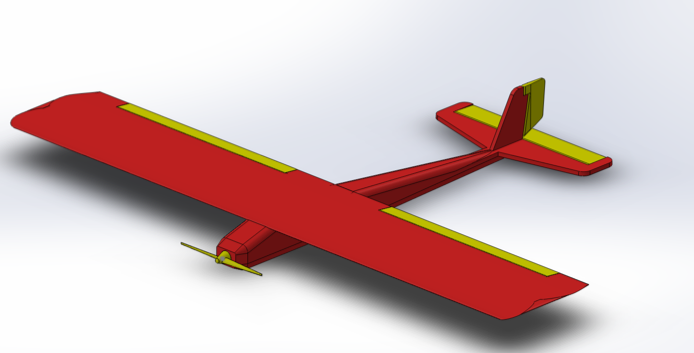
\includegraphics[width=15cm]{allplane.png}
        \end{figure}
        
        \vspace{0.8cm}
        
        University of Sheffield\\
        31th November 2017
        
    \end{center}
\end{titlepage}

\newpage

\begin{landscape}
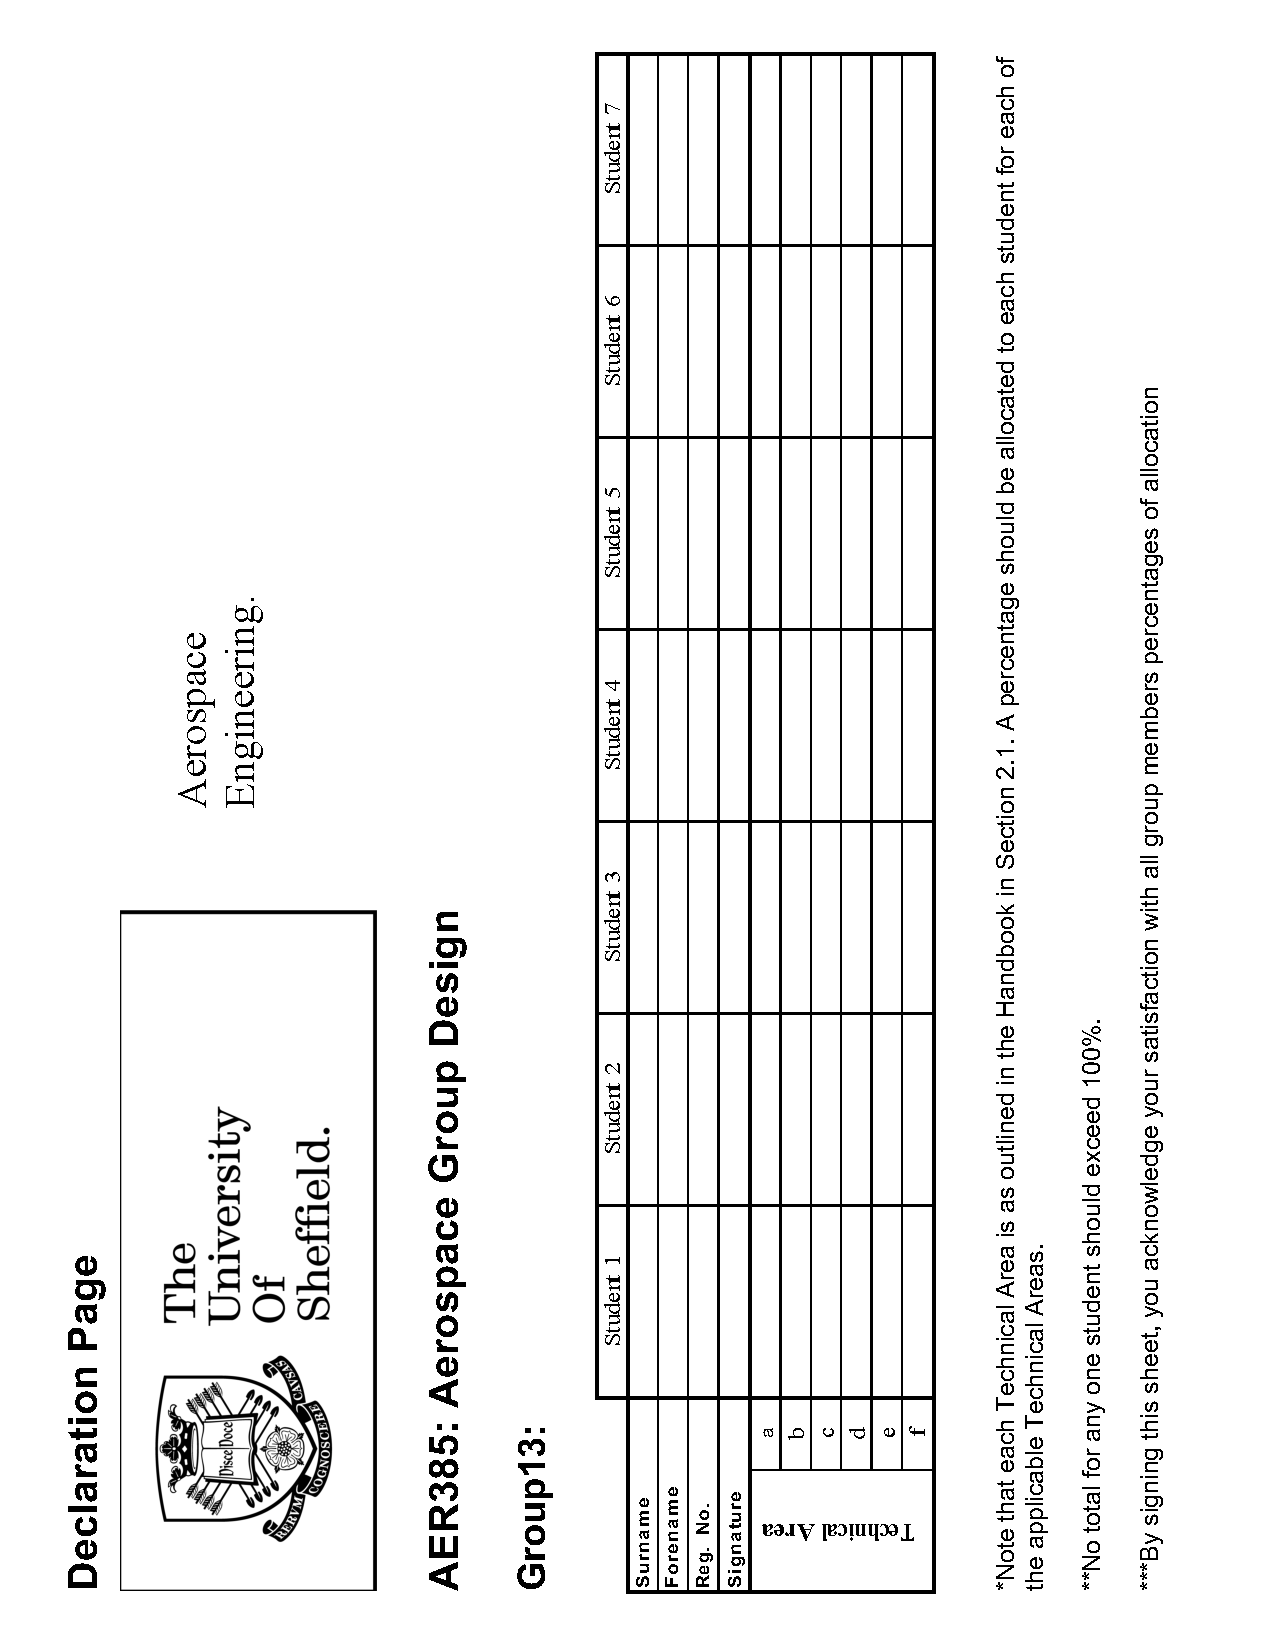
\includepdf[pages=-]{AER385.pdf}
\end{landscape}

\tableofcontents

\newpage

\section{Aims and Requirements}

\subsection{Aims}

\noindent The main aim of the team is to design a fully functional and stable unmanned aerial vehicle (UAV) that shall record aerial photography and/or video and its geographical position can be controlled via GPS. The main requirements that are imposed on the UAV design are stated below. \\

\subsection{Aims and Design Requirements}

\begin{itemize}
    \item The design shall not include a rotating wing.
    \item The design shall not be pressurised.
    \item The design shall meet all the appropriate legislations for operation in the UK.
    \item The UAV shall be easy to maintain and modular so that components can be replaced easily if broken or as upgrades become available.
    \item No single disassembled dimension shall excheed 1.0 meters. 
    \item The overall mass of the UAV shall not be greater than 5 kilograms. 
    \item The UAV shall have an electrical propulsion system.
    \item The UAV shall be capable of being assembled in less than 10 minutes, with minimal available tools and/or in remote locations.
    \item The UAV shall have a minimum endurance of 30 minutes without recharging, considering various flight segments (i.e. take-off, steady flight, landing).
    \item The team shall not exceed the $\pounds$ 850 budget or use any external sponsorship. 
    \item The ground station shall work on standard laptop or tablet.
\end{itemize}

\subsection{Operational Requirements}

\begin {itemize}
   \item The design shall be operating in a non-ideal environment, subject to wind and low levels of rain.
   \item The UAV shall be stable and capable of being operated by someone with minimal training. 
   \item The UAV shall take detailed pictures of the ground during flight. 
   \item The UAV shall continually report to the ground station the following data: current location, battery level and live video feed. 
   \item The autopilot shall autonomously identify 4 different GPS coordinates: pilot coordinates, coordinate boundaries (1, 2, 3 \& 4) and landing zone. 
\end{itemize}

\newpage

\section{Project Planning}

\subsection{Work Breakdown Structure - An Introduction to the Team}

\setlength\arrayrulewidth{0.7pt}
\begin{table}[!htpb]
    \begin{tabular}{ |c| }
        \hline
        \textbf{Thomas Osland}\\
        \hline
        \makecell[tl]{\textbf{Role:} Aerodynamic Team \& Structures, Group13 Team Leader\\ \textbf{Description:} Used CAD design, ANSYS fluent, and Matlab in order to \\
         design the aerodynamics and propulsion of the aircraft. Strong application \\ of aircraft design theory to accurately engineer and optimise the \\ aircraft.}\\
        \hline
        \textbf{Ana-Maria Badilita} \\
        \hline
        \makecell[tl]{\textbf{Role:} Material \& Structure Team Member \\ \textbf{Description:} Experience in CAD \& EXFOIL analysis, Extensive \\ knowledge in manufacturing and material selection processes, \\ Interested in composite materials and additive manufacturing \\ LaTeX support} \\
        \hline
        \textbf{Hamza Bouhouch} \\
        \hline
        \makecell[tl]{\textbf{Role:} Propulsion Team, Control, Sensors, Actuators \& Communicators \\ \textbf{Description:}Extensive knowledge in avionics and electronics, Coding \\ experience in Java \& Python, Experience in CAD Modelling, In charge of \\ actuations, autopilot and propulsion system } \\
        \hline
        \textbf{Arthur Cunningham} \\
        \hline
        \makecell[tl]{\textbf{Role:} Ground Station \& Communications, Control \& Actuations \\ \textbf{Description:} Extensive knowledge inavionics, Overseeing the general \\ avionics along with Hamza, Mainly focused on ground station and control} \\
        \hline
        \textbf{Tobias Sandin} \\\hline
        \makecell[tl]{\textbf{Role:} Aerodynamics \\ \textbf{Description:} Use of Solidworks, Ansys Fluent, \& Matlab to evaluate\\ the range of possible NACA aerofoils through CFD analysis.}\\
        \hline
        \textbf{Samuel Vazquez} \\
        \hline
        \makecell[tl]{\textbf{Role:} Aerodynamic Team \\ \textbf{Description:} Profficient in CAD Modelling and Ansys Fluent, Strong \\ knowledge and understanding of the aircraft design steps} \\
        \hline
        \end{tabular}
    \caption{Group13 Team Members Profiles}
\end{table}

\newpage

\subsubsection{Schedule}

The project can be divided into 2 main phases: semester 1 \& 2; the table below shows the target tasks up to the first module deadline and the current status of the key activities that are currently finalised, in progress or upcoming. The Gantt Chart below explains some of the key activities taking place during the current stage and the people in charge of them. \\

\begin{figure}[hptb]
    \centering
    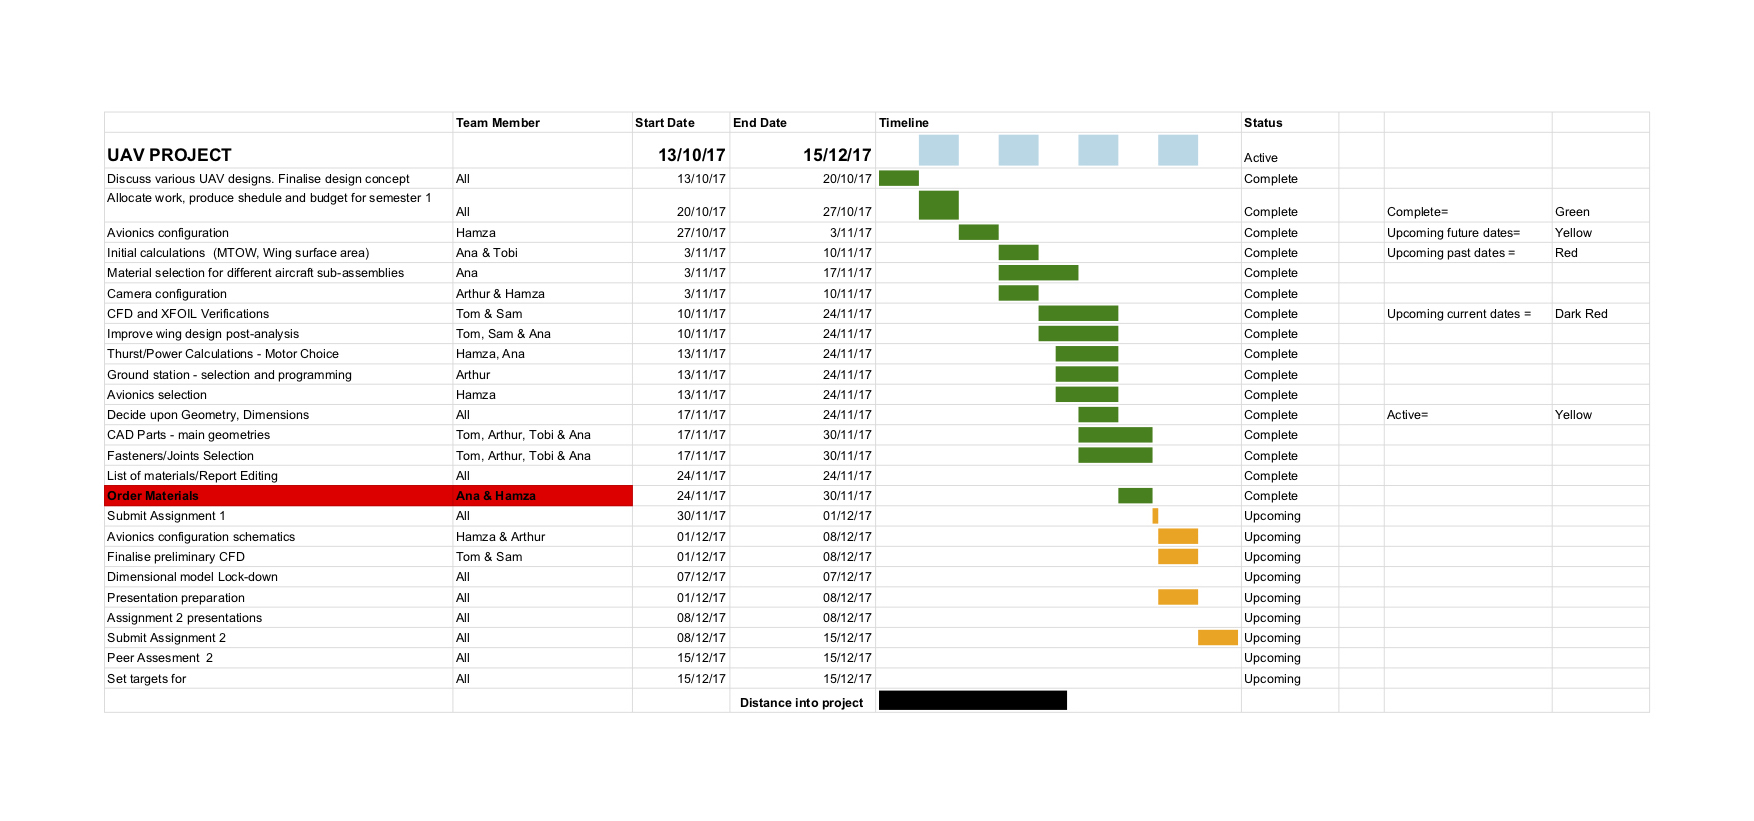
\includegraphics[height=83mm, angle=90, scale=1]{Gannt_Chart_Rotated.jpg}
    \caption{Team13 Gantt Chart}
\end{figure}

\newpage

\subsection{Budget}

\noindent A limited budget is one of the main constraints of the project. Thus, a budget tabel for avionics (including the optional components) has been  created in order to keep track of the components that require immidate purchase. A future material table estimating the expected costs will be included once the material selection process has been finalised.\\

\begin{longtable}{ | c | c | c |} 
    \hline
    \makecell{\textbf{Components}}  & \textbf{Quantity} & \makecell{\textbf{Price} \\ \textbf{($\pounds$)}}\\ 
    \hline
    \endfirsthead

    \hline
    \textbf{Components} & \textbf{Quantity} & \makecell{\textbf{Price} \\ \textbf{($\pounds$)}}\\
    \hline
    \endhead

    \textbf{PIXHAWK} & 1 & 119 \\ 
    \hline
    \textbf{Camera} & 1 & 29.99 \\ 
    \hline
    \makecell{\textbf{Official OSD} \\ \textbf{Board PIXHAWK}} & 1 & 45.95 \\ 
    \hline
    \makecell{\textbf{Cheaper Option} \\ \textbf{OSD Board}} & 1 & 7.50 \\ 
    \hline
    \makecell{\textbf{Video Receiver} \\ \textbf{(5.8 Ghz)}} & 1 & 14.99 \\ 
    \hline
    \makecell{\textbf{Easy CAP} \\ \textbf{Capture USB}} & 1 & 19.99 \\ 
    \hline
    \makecell{\textbf{Transmitter for} \\ \textbf{FUTABA} \\ \textbf{+} \\ \textbf{ENCODER}} & 1 & 27.98 \\ 
    \hline
    \textbf{GPS + Compass} & 1 & 21.99 \\ 
    \hline
    \textbf{APM Module} & 1 & 14.99 \\ 
    \hline
    \textbf{Video Transmitter} & 1 & 14 \\ 
    \hline 
    \textbf{Telemetry Kit} & 1 & 49.99 \\ 
    \hline
    \textbf{Battery} & 1 & Provided\\ 
    \hline
    \makecell{\textbf{Battery Monitor \textbackslash } \\ \textbf{Alarm 1-8S}} & 1 & 3.99 \\
    \hline
    \underline{\textbf{SERVOS/MOTORS}} & & \\ 
    \hline
    \textbf{Tail Plane SERVOS} & 1 & 7.99\\ 
    \hline
    \textbf{Flaps SERVOS} & 1 & 7.99\\ 
    \hline 
    \textbf{SERVOS Setup} & 1 & 7.99\\ 
    \hline
    \textbf{ECS/Motor} & 1 & 7.99\\ 
    \hline 
    \underline{\textbf{OPTIONAL COMPONENTS}} & 1 & \\ 
    \hline
    \textbf{I2C Board} & 1 & 1.99 \\ 
    \hline
    \textbf{LED + USB Module} & 1 & 6.75 \\ 
    \hline
    \textbf{Airspeed Sensor} & 1 & 20.99 \\ 
    \hline
    \makecell{\textbf{Video Transmitter} \\ \textbf{Battery}} & 1 & 7.95 \\ 
    \hline
    \textbf{Total} & 1 & 357.97\\ 
    \hline
    \caption{Avionics Costs}\\
\end{longtable}

\subsection{Law and Safety}

\paragraph {Avionics and Electronics} One consideration that has been imposed was that the frequencies that we were transmitting on may be subject to law or licensing issues. After further research, it was found that the UAV would be classified in the eyes of the law as a ‘Short range device’ (SRD) - description given to “devices such as alarms, telemetry and telecommand devices, radio microphones, radio local area networks and anti-theft devices with maximum powers of up to 500mW at VHF/UHF, as well as certain microwave/Doppler devices with maximum powers of up to $10W$”. This means that the UAV is just within the bounds of an SRD as the highest power that it will transmit at is $500mW$. Thus, it should not need to be licensed.\cite{REFERENCE1} \\

\noindent It also states in the Futaba T6K manual that "To comply with FCC RF exposure compliance requirements, a separation distance of at least $20cm$ must be maintained between the antenna of this device and all persons".\cite{REFERENCE2} \\

\noindent FCC stands for Federal Communications Commission and, although this is an American regulatory body rather than a British one, the team feels that in the interests of safety, it will be observed at all times. \\

\section{Initial Design}

\subsection{Conceptual Design}
\noindent The initial design approach was for the aircraft to be a simple design, making use of concepts which are known to be successful. Research was conducted to investigate low-speed, stable trainer aircraft, designs such as the Cessna 172 Skyhawk (Figure \ref{fig:cessna}). The main design traits discovered were: 

\begin{itemize}
\item{High wing --- for roll stability}
\item{Single front propeller --- for thrust stability}
\item{Inverse T tail --- for lateral stability}
\end{itemize}

\begin{figure}[h]
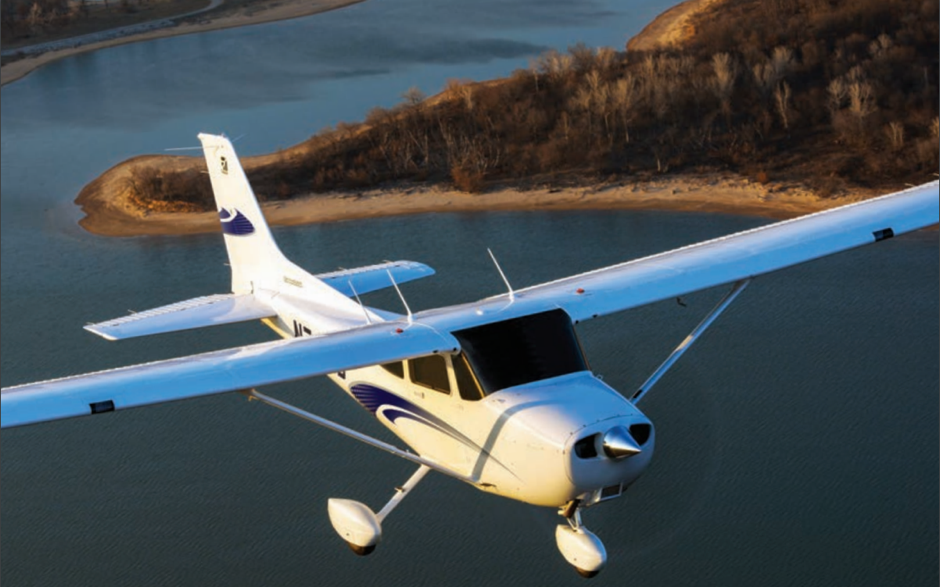
\includegraphics[width=\columnwidth]{cessna.jpg}
\centering
\caption{Cessna 172 Skyhawk}
\label{fig:cessna}
\end{figure}

\noindent Further investigations of full size aircraft led to the research of model trainer aircraft. \cite{TRAINERREF} This revealed similar traits on all the model aircraft proving this to be an effective design aspiration. Concluding these conceptual design observations, it lead to the initial sketch in "First Draught" of what shape and direction the aircraft will take. \\

\subsection{Preliminary Design Review}

\subsubsection{Aerodynamics}

\noindent The Aerodynamics section of this report will identify the key processes for creating the optimum Preliminary Design by considering the key features, such as streamlining, control surfaces and lift devices. These features of the aircraft can be developed once the performance environment has been calculated; this will include take-off, stall and cruise speeds as well as the maximum take-off weight. \\

\paragraph{A. First Draught} For the first design concept, the initial design ideas and constraints were combined to form the CAD model shown in figures below. \\

\begin{figure}
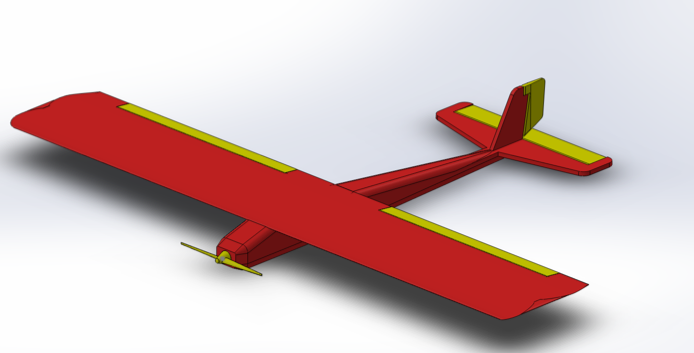
\includegraphics[width=15cm]{allplane.png}
\caption{UAV Orthographic View}
\end{figure}

\begin{figure}
    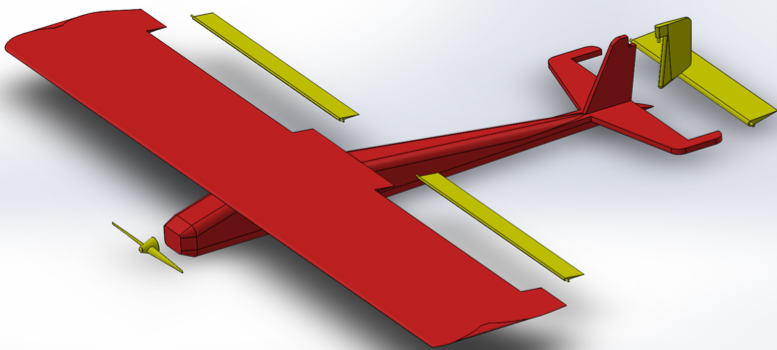
\includegraphics[width=15cm]{allplanedes.png}
    \caption{UAV Exploded View}
\end{figure}


\begin{figure}[h!]
    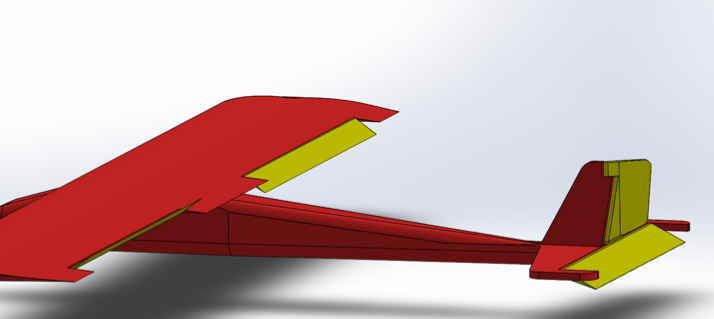
\includegraphics[width=14.5cm]{control.png}
    \caption{Attached Control Surfaces}
\end{figure}

\begin{figure}[h!]
    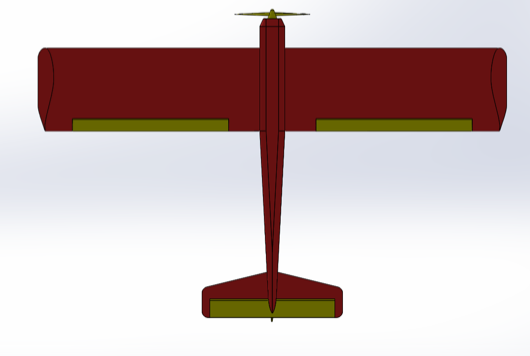
\includegraphics[width=14.5cm]{bottom.png}
    \caption{Bottom View of the UAV}
\end{figure}

\begin{figure}[h!]
    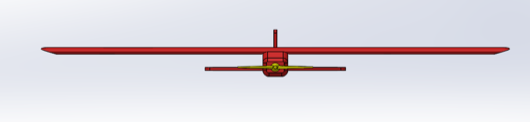
\includegraphics[width=14.5cm]{front.png}
    \caption{Front View of the UAV}
\end{figure}

\noindent It features the stable trainer aircraft characteristics of a high wing, inverse t-tail and single front propeller - all scaled to fit into our design brief. The brief states that no part of the disassembled aircraft can be over $1m$. It was decided that the wing span would be $1.5 m$, constructed out of two parts that would be joined for final assembly and the chord length would be at $0.266    m$ to give a favourable aspect ratio of 7.5. The main fuselage extends $0.943m$. \\

\paragraph{B. Optimisation} Once all initial design objectives had been fulfilled, focus was aimed at optimising the design to ensure the best preliminary design possible. The 4 main points that were addressed were the sizing and details of the wing, wing tips, streamlining and the control surfaces. These four points set out to improve the overall performance of the aircraft by tackling the most significant details in the design. The initial drawing and values gave a base to work upon to then refine each part of the aircraft to create the most optimum design. \\

\paragraph{C. Aifoil Selection}
The typical approach of selecting an airfoil for the wing design is to calculate the ideal lift coefficient and maximum lift coefficient, and map them in the $Cl_{max}$  vs. $Cl_{ideal}$ graph. The governing equations for estimating those two design parameters are: \\

\begin{equation}
    Cl_{ideal} = \frac{2 * W_{avg}}{\rho * V_c^2 * S}
\end{equation}  

\begin{equation}
    Cl_{max} = \frac{2 * W_{TO}}{\rho * V_s^2 * S}
\end{equation}  

\noindent %where $W_{avg}$ is the average weight (in this case as there is no variation in mass, the average mass is equal to the estimated weight of the UAV), WTO is the maximum take-off weight, $V_{c}$ is the cruise speed (the cruise speed was assumed to be 25 m/s),  is the stall speed (the stall speed was assumed to be 10 m/s), $C_{s}$ is the air density at the cruise altitude (in this case, as the altitude range is limited to 10-30 meters above the Earth’s surface, the air density can be assumed constant, having a value of 1.225 $kg/m^2$) and S is the wing surface area. \\

\noindent Thus, the wing surface area is to be calculated. In the current design, the wing is assumed to be rectangular in shape. Thus, for a rectangular wing, the surface area is given by: 

\begin{equation}
    S = b * c
\end{equation}

\noindent %where b is the span (based on the design requirements stated in Section 3.2.1., the maximum span is assumed to be 1m), c is the mean chord (considering a rectangular wing, the chord does not vary between the tip and the root of the wing).\\

\noindent The initial approach was based on varying the chord length (c). The inconsistencies present in scaling a rectangular wing model to a small-size UAV and those due to the innapropriate use of the flow similarity approach generated unreliable results, generating a highly irregular flow around the airfoil. \\

\noindent The second design approach was based on varying the wing surface area in order to estimate the Cube Wing Loading (CWL) given by: 

\begin{equation}
    CWL = \frac{W/S}{sqrt{S}}
\end{equation}

\noindent The cube wing loading generates a number which characterises the wing, comparing the modelled wing with models similar in wing designs and load distribution. Table \ref{table:wcl} gives typical values for various types of aircrafts. \\

\begin{table}[htpb]
    \begin{tabular}{ | c | c |} 
    \hline
    \makecell{\textbf{Type of Aircraft}} & \textbf{Cube Wing Loading} \\ 
    \hline
    Glider & $<$ 4\\ 
    \hline
    Trainers & 6 to 7\\ 
    \hline
    Aerobatics & 9 to 10 \\ 
    \hline
    Scale & 12 to 13 \\ 
    \hline
    Racers & 5 $<$ \\ 
    \hline
    \end{tabular}
    \caption{Typical Wing Cube Loading Values}
    \label{table:wcl}
\end{table}

\noindent By choosing wing areas between $35 - 44dm^2$, the maximum and ideal lift coefficients have been calculated. The aerofoils to be tested further were chosen to be the NACA 64-208, NACA 65-210 and the NACA 65-212, as seen in  Figure \ref{fig:nacas}. These aerofoils were chosen for the higher end of the weight assumptions (e.i. $2.6kg$, $2.8kg$ and $3kg$), allowing for the greatest amount of freedom in further design. The wing area was fixed at $0.4m{^2}$. In the initial wing selection, a span of $1m$ was assumed. However, different length wings hold different properties so the effect of aspect ratio was investigated. This approach produced the following results: NACA63-221, 64-208, 65-210, 65-212 \& 66-218. \\


\begin{figure}[h]
    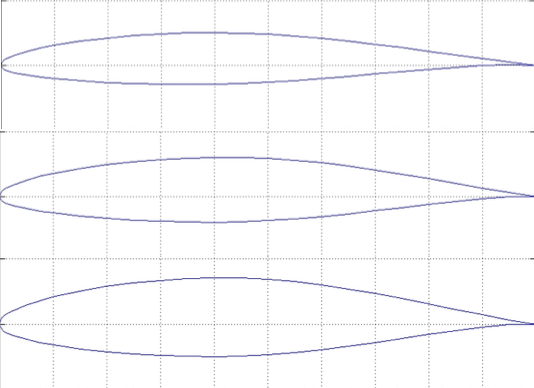
\includegraphics[scale=1]{NACAs.png}
    \centering
    \caption{(From top to bottom) NACA 64-208, NACA 65-210 and NACA 65-212}
    \label{fig:nacas}
\end{figure}

\noindent The last approach involved the use of the XFOIL software in designing the airfoil and simulate the airflow around the wing section. The student version of XFOIL can only generate the NACA 4-digit \& 5-digit series. \\

\noindent For the 5-digit series, the first digit can only be 2 (therefore, the airfoils previously selected could not be simulated in XFOIL); this value corresponds to a design lift coefficient of approximately 0.3. \\

\noindent The second and third digits correspond to the maximum camber and its position in relation to the chord line. For the simplicity of the design during manufacturing, the camber has been varied between values of 5 and 15; the camber improves the lift generation for each angle of attack. Therefore, in order to maximise the lift coefficient, a cambered airfoil design was preferred). \\

\noindent The last two digits are the thickness-to-chord ratio expressed as a percentage. The thickness was varied between 10 and 12, as for any value bigger than 14, the thickness will generate less lift and higher drag. \\

\noindent For the 4-digit series, the first two digits correspond to maximum camber and the position of the maximum camber relative to the chord line, respectively, while the last two digits correspond to the thickness-to-chord ratio, again expressed in the form of a percentage. Typically, the 4-digit NACA airfoils produce more drag compared to the new 5-digit and 6-digit series. However, based on the simulations, for the current design, they produce a little more lift. The maximum camber was assumed to be equal to 2, while the position has been varied from 20\% to 30\% of the chord length. Again, the thickness-to-chord ratio values have been either 13 or 14. \\

\noindent As XFOIL simulates the airfoil around a 2D body, the aspect ratio can be changed, changing the flow regime (i.e. the Reynolds number). Based on the second approach, the optimum chord length is between $30 - 40cm$. Thus, the Reynolds number has been calculated using Equation \ref{eq:rey} and, giving the chord values between $30 - 40cm$.

\begin{equation}
    Re = \frac{\rho * u * c}{\mu}
    \label{eq:rey}
\end{equation}

\noindent With increased thickness, up to 12\%, more lift is generated, with a very reduced increase in drag. Considering the highest lift coefficient and lowest drag coefficient that have been produced (the values generated are between 0.079 and 0.1172 for the lift coefficient \& 0.000654 and 0.00084 for the drag coefficient), the following airfoils have been considered optimal: NACA23011 and NACA2313. \\

\begin{figure}[h]
    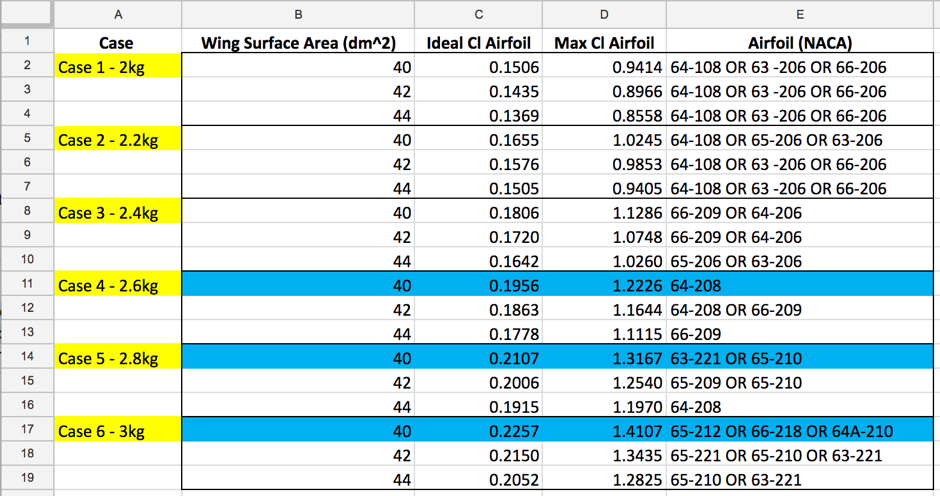
\includegraphics[width=\columnwidth]{aerofoilchoice.png}
    \centering
    \caption{Aerofoil Calculations}
    \label{fig:aerofoilcalc}
\end{figure}

\noindent The main assumptions made in these analysis are the following: \\

\begin{itemize}
    \item $V_{stall} = 10 m/s$ (stall speed);
    \item $V_c = 25 m/s$ (cruise speed);
    \item $\rho = 1.225 kg/m^3$ (the air density is assumed fairly constant as the change is altitude is reduced to a range of 10-30 meters);
    \item $\mu = 1.857*10_{-5}kg/(m*s)$ 
    \item the chord length varies between 25 and 40 cm;
    \item the Reynolds number has values of 510000, 600000 and 610000. 
\end{itemize}

\paragraph{D. Aspect Ratio} To find a suitable aspect ratio, the lift induced drag and Reynolds number over a range of aspect ratios were investigated at cruise conditions. The cruise speed chosen was $25ms{{^-}^1}$.  Lift induced drag is the drag produced as a result of generating lift and acts perpendicular to the direction of lift. It is directly linked to the aspect ratio which can be seen within Equation \ref{eq:cdi}. The span efficiency factor $e$ was assumed to be 0.9. 

\begin{equation} \label{eq:cdi}
    C{{_d}_i} = \frac{C_L^2}{\pi*e*AR}
\end{equation}

\noindent The coefficient of lift used in Equation \ref{eq:cdi}  was calculated using Equation \ref{eq:cl}. At cruise conditions, the lift is equal to weight. 

\begin{equation} \label{eq:cl}
    C{_L} = \frac{2*L}{\rho*{V^2}*S} = \frac{2*W}{\rho*{V^2}*S}
\end{equation}

\noindent The lift induced drag coefficient for various aspect ratios and weights of aircraft can be seen within Figure \ref{fig:DragvAR}. \\

\begin{figure}[h]
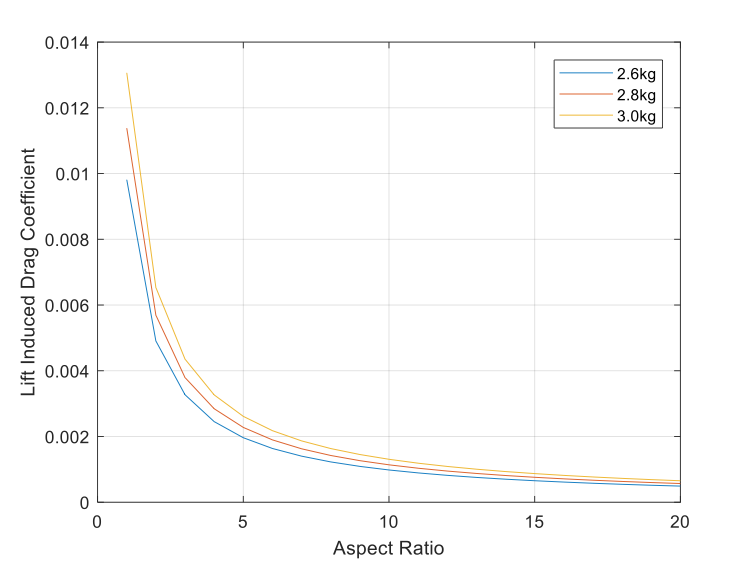
\includegraphics[width=11cm, scale=1]{DragvAR.png}
\centering
\caption{Lift Induced Drag Coefficient for Various Aspect Ratios, at Varying Mass}
\label{fig:DragvAR}
\end{figure}

\begin{figure}[H]
    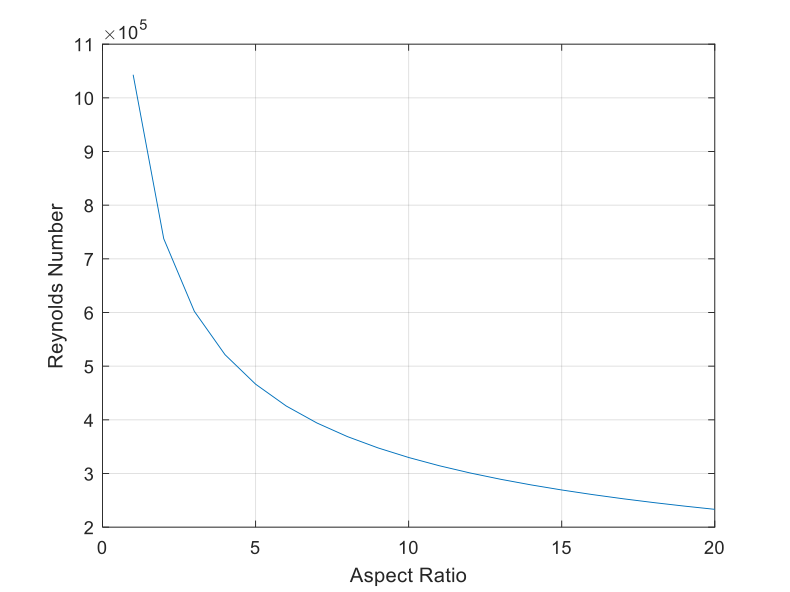
\includegraphics[width=11cm, scale=1]{ReVAR.png}
    \centering
    \caption{Reynolds Number at Various Aspect Ratios}
    \label{fig:ReVAR}
\end{figure}

\noindent Figure \ref{fig:DragvAR} shows that the lift induced drag reduces as the aspect ratio increases. This is because at a greater aspect ratio, the chord becomes shorter which leads to smaller wing tip vortices. Alongside this, as the weight increases, so does the lift induced drag, due to requiring a greater amount of lift. The aspect ratio also directly affects the Reynolds number. \\

\noindent Figure \ref{fig:ReVAR} shows that the Reynolds number decreases as the aspect ratio increases, due to the shorter chord length. Having a low Reynolds number means there are stronger viscous effects which leads to increased frictional drag. It is also more prone to boundary layer separation and laminar separation bubbles. Therefore, having a suitably high Reynolds number aids performance. Due to this, an aspect ratio had to be chosen that suitably reduces lift induced drag and keeps a satisfactory Reynolds number. Accounting for this, a span of $1.5m$ was chosen, which corresponds to an aspect ratio of 5.64. The chord to match this was $0.266m$. The lift induced drag coefficient for various weights can be seen within Table \ref{table:indrc}. \\

\begin{table}[h]
    \centering
    \begin{tabular}{|l|c|}
        \hline
        \textbf{Mass} & \textbf{Lift Induced Drag Coefficient, $C{{_d}_i}$} \\
        \hline 
        $2.6kg$ & $0.0017$ \\
        \hline 
        $2.8kg$ & $0.0027$ \\
        \hline 
        $2.9kg$ & $0.0023$ \\
        \hline
    \end{tabular}
    \caption{Lift Induced Drag Coefficient at the Chosen Aspect Ratio for Various Masses}
    \label{table:indrc}
\end{table}

\noindent The Reynolds number is independent of mass and was found to be $4.386*10{^5}$ at the chosen aspect ratio. \\

\paragraph{E. Ansys Simulation} In order to evaluate the range of NACA aerofoils chosen, a 3D simulation was produced within Ansys Workbench to generate key aerodynamic information. The simulation was run for one side of the wing, from the root to the tip. The geometry of the fluid domain can be seen within Figure \ref{fig:cfdgeom}. \\

\begin{figure}[H]
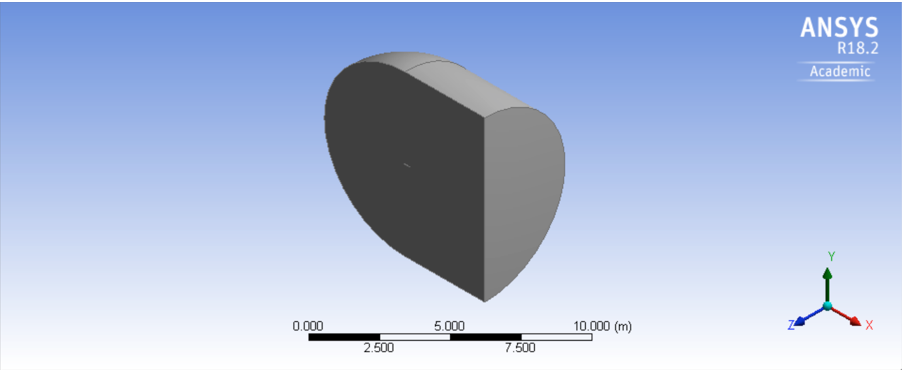
\includegraphics[width=18cm, scale=1]{cfdgeometry.png}
\centering
\caption{Geometry Used in Fluid Simulation}
\label{fig:cfdgeom}
\end{figure}

\noindent Use of this geometry allows analysing the full 3D effect over the wing, whilst easily being capable of altering the angle of attach due to the spherical shape of the inlet surface. \\

\noindent When producing the values for lift and drag on the aerofoil, a number of various models can be chosen, each having their distinct advantages. More complex models with finer convergence criteria can be chosen to achieve more accurate values at the expense of a longer computational time. For the initial 3D modelling, the realizable k-$\epsilon$ (k-epsilon) model was chosen with scalable wall functions. The realizable k-$\epsilon$ is an improvement on the standard k-$\epsilon$ model by containing a new formulation for the turbulent viscosity and a new equation for the dissipation rate, allowing more accurate results. A convergence criteria was also used. \\

\noindent The conditions used can be seen within Table \ref{tabel:spa}. \\

\begin{table}[h]
\centering
\begin{tabular}{|l|l|}
\hline
\textbf{Velocity} &  $25ms{{^-}^1}$
\\ \hline \textbf{Chord Length} & $0.266m$
\\ \hline \textbf{Span (Half of total)} & $0.75m$
\\ \hline
\end{tabular}
\caption{Conditions Used Within Simulation}
\label{tabel:spa}
\end{table}

\noindent By simulating the aerofoils at multiple angles of attack, various properties of the wings can be seen. \\

\begin{figure}[H]
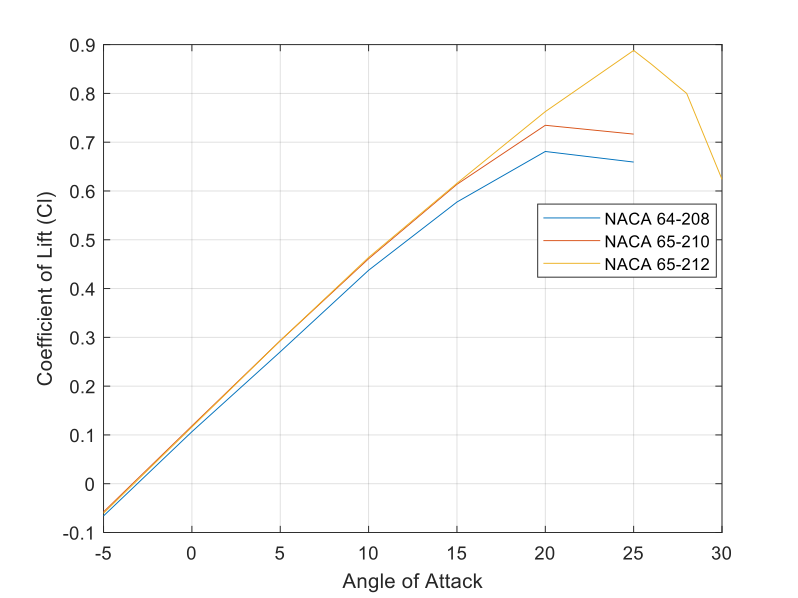
\includegraphics[width=11cm, scale=1]{clvAOA.png}
\centering
\caption{Coefficient of Lift Against Angle of Attack for the Various Aerofoils}
\label{fig:clvAOA}
\end{figure}

\noindent Figure \ref{fig:clvAOA} shows that for low angles of attack, the lift produced by all the designs was very similar. The main distinguishing property for each was the stall angle. Both the NACA 64-208 and NACA 65-212 had similar stall angles, approximately 22$^{\circ}$. The NACA 65-212 had a larger stall angle of 25$^{\circ}$. The 65 series also consistently produced more lift for all angles of attack when compared to the 64 series. By looking where the chart intersects the x-axis, the wing setting angle was seen to be approximately -4 for the NACA 65-210 and 65-212, and -3.5 for the NACA 64-208. \\

\begin{figure}[H]
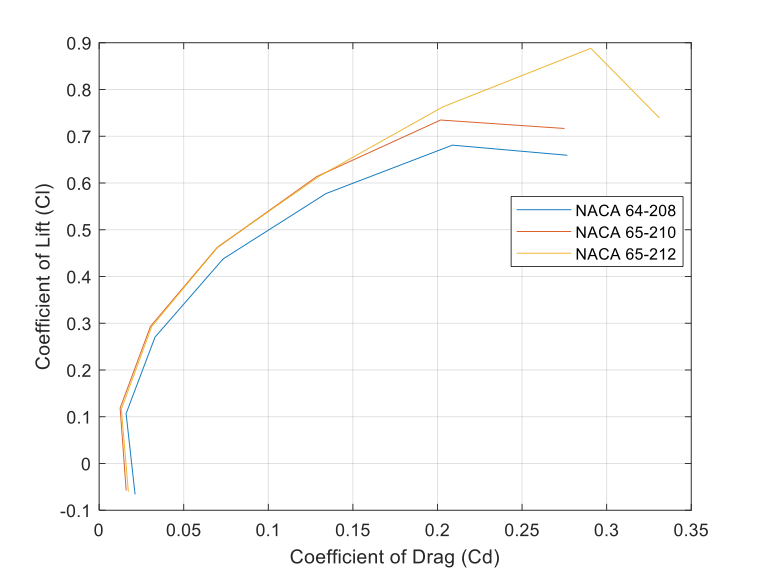
\includegraphics[width=11cm, scale=1]{clvcd.png}
\centering
\caption{Lift/Drag Polar for the Various Aerofoils}
\label{fig:clvcd}
\end{figure}

\noindent Figure \ref{fig:clvcd} shows that the NACA 65-212 and NACA 65-210 had the best aerodynamic efficiency (maximum lift to drag ratio). It is expected that the performance of these aerofoils would be very similar due to only having a slight variance in thickness. At lower levels of lift, the NACA 65-210 marginally produced the least drag, however, at higher values, the thicker 65-212 produced less. Consistently, the 64-208 produced greater drag values. \\

\noindent When looking at the streamlines graphics, one aspect seen throughout all wing designs was the effect of wing tip vortices. This can be visualised in Figure \ref{fig:nac65212}. \\

\begin{figure}[H]
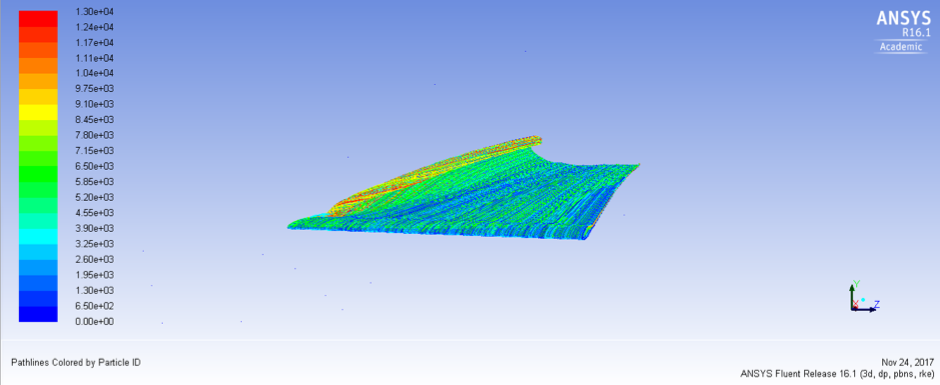
\includegraphics[width=18cm, scale=1]{naca65212streamline.png}
\centering
\caption{Streamline Graphic for the NACA 65-212 at 10 Degree Angle of Attack}
\label{fig:nac65212}
\end{figure}

\noindent By looking at the wing tip (left edge), the large wing tip vortex can be seen by the curling of the streamlines, as the high pressure air folds around the tip. The vortex would considerably add to the drag for the designs so reducing this would be extremely beneficial to the performance of the aircraft. \\

\noindent Throughout, the NACA 64-208 consistently performed the worst, so was removed from the selection. When comparing the NACA 65-210 and NACA 65-212, both performed very similarly. However, a slightly thicker design is preferable. This would allow for more ease when placing the servos within the wing and also allows for a stronger wing design to be made, reducing the risk of failure in flight. \\

\noindent Figure \ref{fig:pressurecoeff} shows the variation of pressure coefficients over the length the wing. The pressure coefficient is a dimensionless quantity which can show the relative pressure over the wing. It is also directly linked to the coefficient of lift. It is calculated using Equation \ref{eq:p} where $p$ is the pressure at the point on the wing, $p{_\infty}$ is the free stream pressure, and $V{_\infty}$ is the free stream velocity.

\begin{equation} \label{eq:p}
C{_p} = \frac{p-p{_\infty}}{\frac{1}{2}*p{_\infty}*V{^2_\infty}}
\end{equation}

\noindent It can be seen that the pressure at the leading edge and the first third of the wing experiences the greatest pressure; so ensuring strength in this particular section of wing in manufacture is key in ensuring that the wing doesn’t fail in flight. It is also here where the greatest amount of lift is produced. \\

\begin{figure}[H]
    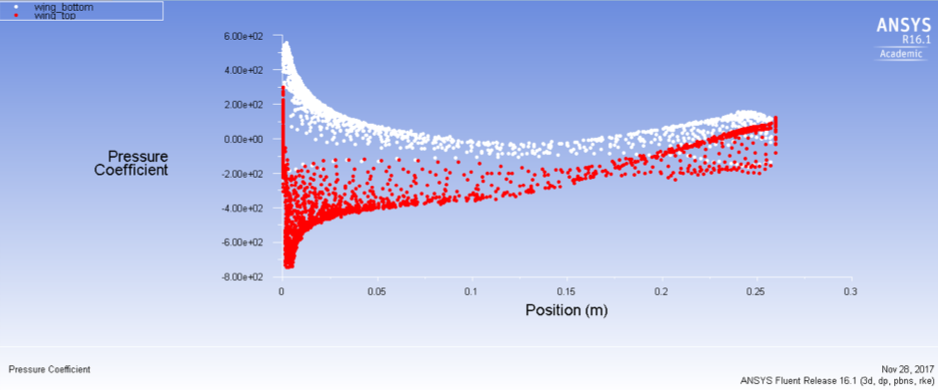
\includegraphics[width=18cm, scale=1]{pressurecoeff.png}
    \centering
    \caption{Pressure Coefficients on the NACA 65-212 at 10 Degrees Angle of Attack}
    \label{fig:pressurecoeff}
\end{figure}

\paragraph{F. Speed Calculations} The stall, take-off and cruise speeds have been estimated as part of the preliminary design. \\

\noindent \textbf{1. Stall Speed}
\noindent Using the Lift equation, the stall speed is able to be calculated once the max coefficient of lift is calculated; from the analysis, $C{{{{{_L}_m}_a}_x}}$ is 0.9. Therefore the following calculation is produced:

\begin{equation} \label{eq}
V{_stall} = \sqrt{\frac{2*m*g}{\rho *S* C{_L}}}
\end{equation}

\noindent \textbf{2. Take-Off Speed}
\noindent The Rotation Velocity, $V{_R}$, otherwise known as the take off speed, should be 1.2 times that of the stall speed. This gives us $V{_R} = 13.86ms{{^-}^1}$.\cite{TAKEOFFREF} \\

\noindent \textbf{3. Cruise Speed}
\noindent The desired cruise speed of our UAV is $25ms{{^-}^1}$. In order for this to be successfully carried out, the cruise angle of attack has to be calculated, but this cannot be done without knowing the required cruise coefficient of lift.

\begin{equation} \label{eq}
C{_L} = \frac{2*m*g}{\rho * V{^2}*S} = \frac{2*3*9.81}{1.225*25{^2}*0.4} =0.19
\end{equation}

\noindent This required $C{_L}$ can be acquired on the $C{_L}$  vs AOA figure, which translates to an angle of attack at 3 degrees. This means that when the aircraft wishes to cruise at $25ms{{^-}^1}$, then it must travel at a 3 degrees AOA. \\

\paragraph{G. Sizing Of Tail} Surface areas of the vertical and horizontal tail parts are directly linked to the main wing geometry and position of the tail, as the tail must counter moments created by the wing while in flight. For initial estimations of the tail size, the tail volume coefficient approach was used. This links the surface area of the horizontal and vertical tail sections to the distance of the tail moment around the entre of mass and some of the main wing geometry. The tail volume coefficient can be found in tables, detailing typical values for different types of aircraft. For this aircraft, the values for horizontal and vertical tail volume coefficients were chosen as 0.4 and 0.02 respectively. Equations \ref{eq:sh} and \ref{eq:sv} were then used to calculate an initial estimate for surface areas for the horizontal and vertical tails. \\

\begin{equation} \label{eq:sh}
V_H = S_H * L_H/S_W * m.a.c
\end{equation}

\begin{equation} \label{eq:sv}
V_V = S_V * L_V/S_W * b
\end{equation}

\begin{figure}[H]
    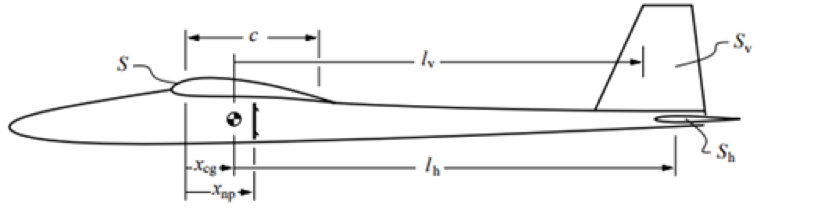
\includegraphics[width=18cm, scale=1]{tailsize.png}
    \centering
    \caption{Sizing of Tail\cite{TAILSIZEREF}}
    \label{fig:tailsize}
\end{figure}
    
\noindent These gave values of $S{_v}=0.01689m{^2}$ and $S{_h}=0.05992m{^2}$ which were then implanted into the design. Although these values are much larger than on the original conceptual design (i.e. less aerodynamic), the calculations indicate that these new values are necessary to ensure the stability of the aircraft in flight. \\

\noindent From an aerodynamic standpoint, the changes made between the first itiration to the current design can be evaluated using CFD analysis. Using similar techniques as to those in the analysis of different aerofoils, the flow can be modelled over the entire aircraft in both cases. For this set of simulations, the values of cruise velocity and angle of attack were used. \\

\noindent Figures \ref{fig:pressbad} and \ref{fig:pressgood} show the differences in pressure coefficients around the aircraft’s main body and over midsection. From this it can be seen that the large concentration of high pressure coefficient at the nose has been reduced significantly in the final design. Furthermore, the pressure coefficient profile over the final design’s wing section is more pronounced, indicating a larger pressure difference over the wing; so, more lift is generated. These differences are due to streamlining on the main fuselage and the change in the aerofoil section, from NACA 0012 to NACA 65-212. \\

\begin{figure}[h!]
    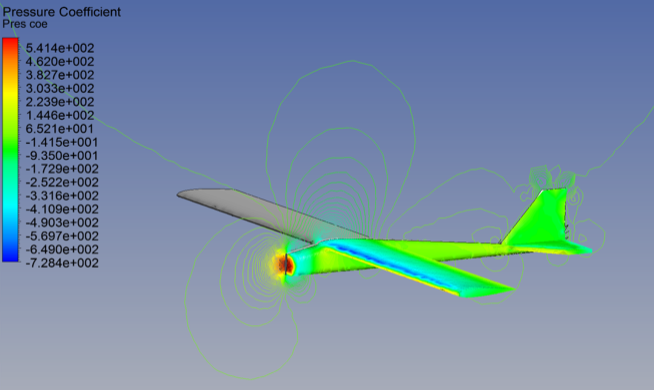
\includegraphics[width=13cm, scale=1]{Pressurecoefficientbad.png}
    \caption{Pressure Gradient of NACA0012}
    \label{fig:pressbad}
\end{figure}

\begin{figure}[h!]
    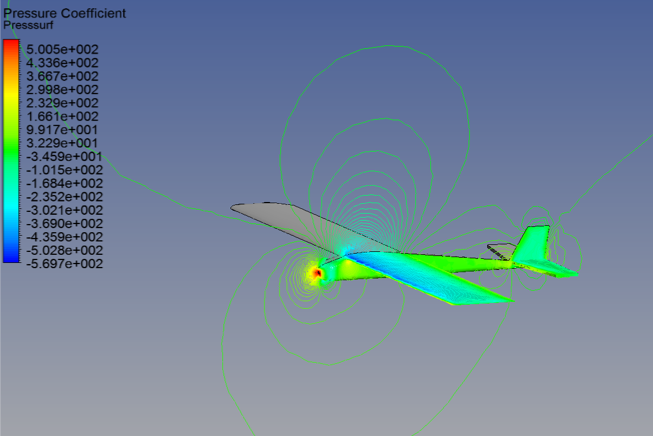
\includegraphics[width=13cm, scale=1]{pressurecoeffientgood.png}
    \caption{Pressure Gradient of NACA65-212}
    \label{fig:pressgood}
\end{figure}

\noindent Figure \ref{fig:vel} shows the velocity over the midsection of the aircraft. Similar differences can be seen here over the wing sections of both designs. The blue zones on the first draft (Figure \ref{fig:velbad} indicate areas where airflow has slowed significantly. This is fine on the aircraft’s surface, however this happens in quite large areas on the first draft’s nose tip showing some streamlining issues. This problem has been solved in the final design by redesigning the fuselage. Another blue zone appears behind the wing section on the first draft, which suggests that flow separation has begun and results in a loss of lift. This issue has also been resolved in the final draft with a change in aerofoil design and streamlining of the fuselage. \\

\begin{figure}[h!]
    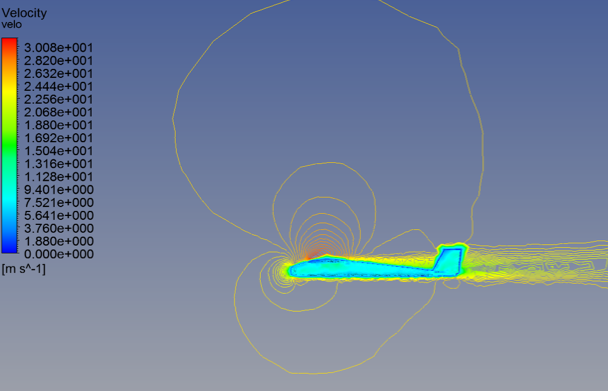
\includegraphics[width=10cm, scale=1]{velocity.png}
    \caption{Velocity Profile NACA65-212}
    \label{fig:vel}
\end{figure}

\begin{figure}[h!]
    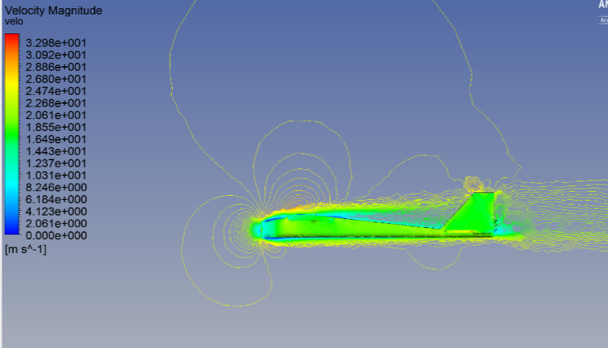
\includegraphics[width=10cm, scale=1]{badvel.png}
    \caption{Velocity Profile NACA0012}
    \label{fig:velbad}
\end{figure}

\noindent From Fluent’s solver, it is possible to extract the values of lift and drag over the entire simulated body. TABLE shows these results and it appears that the final design generates a lot more lift than the initial one. An aircraft of 3kg would need $27.43N$ to stay in steady level flight. Hence, these values of lift show that for the final design, the amount of lift generated would be more than sufficient for an UAV of $3kg$ to stay in the air. These results cannot be taken as a definite truth, as CFD analysis cannot model exactly the dynamic behaviour of the aircraft. This CFD analysis indicates that the steps taken so far to optimise the design have been successful in improving the UAV’s aerodynamic performance. \\

\begin{table}
\begin{tabular}{|c|c|c|}
\hline
\textbf{Design} & \textbf{Lift ($N$)} & \textbf{Drag($N$)} \\
\hline
\textbf{Initial Iteration} & 14.75 & 3.06 \\
\hline
\textbf{Final Iteration} & 32.67 & 2.85 \\
\hline
\end{tabular}
\caption{Lift \& Drag of Two Different Iterations}
\end{table}

\paragraph{H. Wing Tips} Due to the nature of wings generating lift, the higher pressured air on the bottom surface of the wing wants to escape, going to the top surface, and this occurs most noticeably around the wing tips as a vortex is generated. This phenomenon reduces the pressure difference between the two sides of the wing and the wing tip vortices will cause lift induced drag, both creating the effect of a reduced wing span. Adding wing tips can help stop this change of pressures occurring and reduce the effects of the wing tip vortices. \\

\noindent The 4 wing tip types that were investigated by CFD analysis were: flat tip, rounded tip, winglet and Hoerner tip. Each simulation was run at a cruise velocity of $25m/s$, on half section of the wing, and at an angle of attack of 10 degrees for exaggerated flow behaviour. \\

\noindent The flat tip shows the characteristics to be expected from this type of situation, with a vortex trailing back from the tip. \\

\noindent Rounded tip actually shows to have reduced the effective wing span, as the smoothed tip edges encourages pressure changes over the wing. \\

\begin{figure}[h]
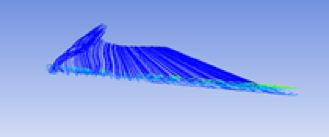
\includegraphics[width=10cm,scale=1]{flattip.png}
\caption{Flat Tip}
\label{fig:flattip}
\end{figure}

\begin{figure}[h]
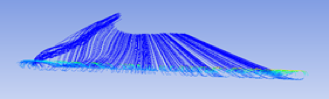
\includegraphics[width=10cm, scale=1]{roundtip.png}
\caption{Rounded Tip}
\label{fig:roundtip}
\end{figure}

\begin{figure}[h!]
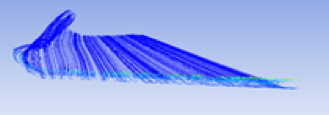
\includegraphics[width=10cm, scale=1]{winglet.png}
\caption{Winglet}
\label{fig:winglet}
\end{figure}

\begin{figure}[h!]
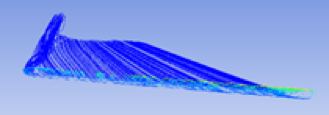
\includegraphics[width=10cm, scale=1]{hoerener.png}
\caption{Hoerner Tip}
\label{fig:hoerner}
\end{figure}

\noindent Winglets shift the tip much further up, which makes it harder for wing tip vortices to form; thus, the lift induced drag is decreased. \\

\noindent From Figure \ref{fig:hoerner}, it is possible to see that the Hoerner tip has moved the vortex to the edge, which would indicate it has increased the effective wing span when compared to the flat tip. From Table \ref{fig:wingdrag}, it is also clear to see that the Hoerner wing tips have the most favourable lift and drag characteristics. \\

\begin{table}[h]
\centering
\begin{tabular}{|c|c|c|}
\hline
\textbf{Wing Tip} &  \textbf{Lift Generated (N)} & \textbf{Drag Generated()N} 
\\ \hline Flat Tip & $41.30$ & $4.54$
\\ \hline Rounded Tip & $41.05$ & $4.47$
\\ \hline Winglet & $41.73$ & $4.49$
\\ \hline Hoerner tip & $41.61$ & $4.46$
\\ \hline
\end{tabular}
\caption{Wing Tips Drag and Lift Values }
\label{fig:wingdrag}
\end{table}

\paragraph{I. Streamlining} Streamlining of the aircraft is important as the shape and size of an object directly affects its coefficient of drag, which in turns affects its coefficient of lift. \\

\noindent Figure \ref{fig:streamline} shows objects with the same frontal area and their coefficients of drag. It shows that as you change the shape to something more streamlined, it reduces the coefficient of drag. This shows that it’s important to ensure a well streamlined aircraft to be designed, as it will reduce the drag and therefore improve the overall performance of the aircraft. \\

\begin{figure}[H]
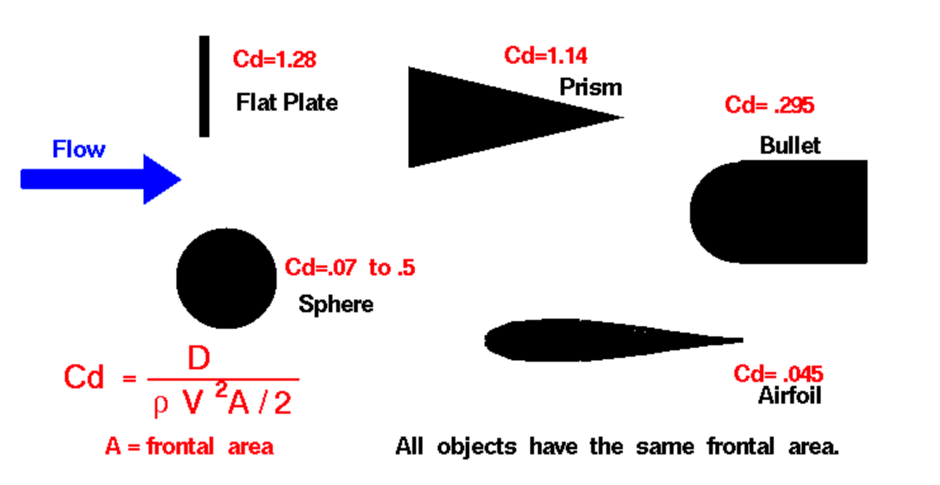
\includegraphics[width=15cm, scale=1]{streamlinenasa.png}
\caption{The Concept of Streamlining \cite{NASAREF}}
\label{fig:streamline}
\end{figure}

\paragraph{J. Aircraft Performance Parameters} Based on the design stages considered in this section, the performance parameters are showed in Table \ref{thing}. 

\begin{table}[h!]
\centering
\begin{tabular}{|l|l|}
\hline
\textbf{Thrust (Minimum)} & $5.66N$
\\ \hline \textbf{Power (Required)} & $202W$ 
\\ \hline \textbf{Velocity --- Cruise} & $25ms{{^-}^1}$ 
\\ \hline \textbf{Velocity --- Stall} & $11.5ms{{^-}^1}$ 
\\ \hline \textbf{Velocity --- Maximum } & $30ms{{^-}^1}$ 
\\ \hline \textbf{Mass (Maximum)} & $3kg$ 
\\ \hline \textbf{Wing Area} & $0.4m^2$ 
\\ \hline \textbf{Wing Span} & $1.5m$ 
\\ \hline \textbf{Chord Length} & $0.266m$ 
\\ \hline \textbf{Aerofoil} & NACA 65-212 
\\ \hline
\end{tabular}
\caption{Aircraft Performance Values}
\label{thing}
\end{table}

\paragraph{K. Aircraft Design Limits} Figure \ref{fig:acdesignreq} shows the boundaries for which the aircraft must remain within the shaded area. The graph was created by understanding all the initial aircraft performance elements, then plotting the aircraft maximum velocity for changing wing loading and thrust to weight ratios. The stall at changing the thrust to weight ratio was also plotted. This left an enclosed area of which the aircraft must lie in order to successfully fly. \\

\noindent The minimum requirement for how heavy the aircraft can be can be calculated using the wing loading equation. The wing loading must be no more than $73.5 N/m^2$ for a stall speed of $11.55m/s$. If the wing area of the aircraft is $0.4m^2$, a currently determined value, then the aircraft must not exceed $3kg$ in order to successfully fly. When manufacturing the aircraft if the total mass increases more than the calculated one, the wingspan will need to be increased. The thrust to weight ratio shows that the minimum power requirement of the aircraft for steady level flight is $202W$, for a mass of $3kg$. This power requirement will be overestimated when choosing a motor to ensure the aircraft will have sufficient power for all flight manoeuvres. \\

\begin{figure}[h]
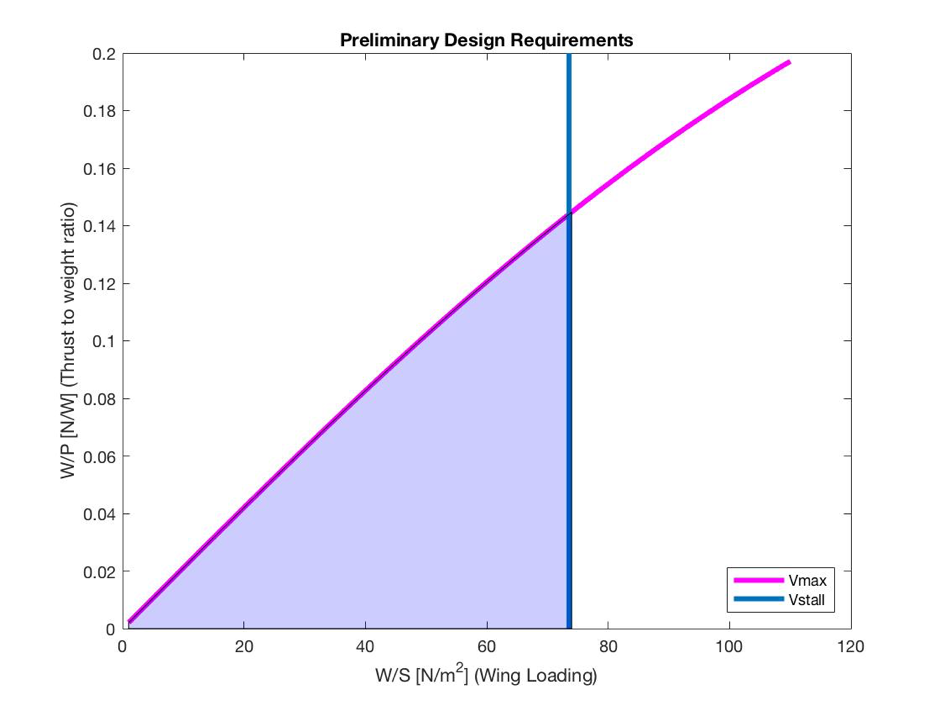
\includegraphics[width=15cm, scale=1]{acdesignreq.png}
\caption{Preliminary Design Requirements}
\label{fig:acdesignreq}
\end{figure}

\newpage

\subsubsection{Propulsion and Electrical Power}

\noindent By inputting the values of cruising speed, wing area and span, weight, coefficient of lift, type of battery (2s, 3.7 V per cell), flight altitude, required thrust, the approximate flight time and  type of mission (acrobatic, trainer etc \ldots), it was possible to obtain some valuable data by using the "eCalc" programme. \cite{ESCREF} This software reaches in its database and, by comparing the different requirements, it is able to create a list of propellers, motors and ESC boards that are able to satisfy our design requirements. In this case, during the design process, the velocity values have been slightly over engineered, to allow us to find a motor that could supply enough power at all times. \\

\noindent Although this approach was successful in creating a complete list, this unfortunately, mostly includes motors that are out of our budget prevision or are not supplied by our authorized suppliers. To find a solution to these issues, the values of speed were slightly lowered to 80-85\% of the original values, leaving us with a larger margin to work with. By doing so in the list of components, an engine size was found; then, by relying on the scheme shown below (Figure \ref{fig:prop}, a propeller size can be selected. 

\begin{figure}[h!]
  \centering
  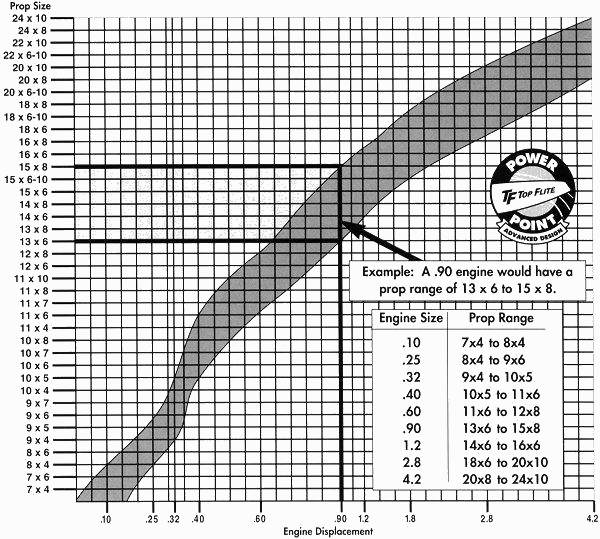
\includegraphics[width=13cm, scale=1]{propscheme.jpg}
  \caption{Propeller Scheme-Engine Size vs. Propeller Size[2];}
  \label{fig:prop}
\end{figure}

\newpage

\subsubsection{Materials and Structure}

\paragraph{A. Materials}
A typical material selection process begins with a “selection matrix”, where the optimum material is chosen in accordance to the best combination of properties, in order to achieve the best performance. However, for the current design, the team members decided to create a hybrid, using all the resources made available as part of the project, such as balsa wood, 3D printed plastics and carbon fibre reinforced composites. Therefore, the different types of material have been engaged in different areas within the design, in order to optimise the price and take advantage of the properties offered by those. \\

\noindent The UAV mechanical structure has been divided in 4 main sub-assemblies: fuselage, wings, tail \& control surfaces and other features. The most suitable materials that can be used for each sub-assembly or part are indicated in Table \ref{tablemat}. \\

\begin{longtable}{ | c | c | c | c |} 
    \hline
    \makecell{\textbf{UAV} \\ \textbf{Sub-assembly}} & \textbf{Part} & \textbf{Material} & \textbf{Type} \\
    \endfirsthead 

    \hline
    \makecell{\textbf{UAV} \\ \textbf{Sub-assembly}} & \textbf{Part} & \textbf{Material} & \textbf{Type} \\
    \hline
    \endhead

    \hline
    \textbf{Fuselage} & \makecell{Round fuselage \& \\ Planked fuselages} & \makecell{Balsa \\ wood} & \makecell{A \\ Grain}\\ 
    \hline
    & Flat fuselage sides & \makecell{Balsa \\ wood} & BGrain\\ 
    \hline
    \textbf{Wings} & Wing leading edges & \makecell{Balsa \\ wood} & \makecell{A \\ Grain}\\ 
    \hline
    & Wing trailing edges & \makecell{Balsa \\ wood} & \makecell{B \\ Grain}\\ 
    \hline
    & Spars & \makecell{Balsa \\ wood} & \makecell{A-Grain}\\ 
    \hline
    & Wing ribs & \makecell{Balsa \\ wood} & \makecell{B/C \\Grain}\\ 
    \hline
    & Wing sheets & \makecell{Balsa \\ wood} & Cgrain\\ 
    \hline
    \makecell{Tail and \\ Control \\ Surfaces}& \makecell{Horizontal \& \\ vertical tail \\ (Option B)} & \makecell{Carbon fibre \\ composite} & \makecell{Carbon fibre \\ reinforced \\ thermoplastic \\ matrix}\\ 
    \hline
    & \makecell{Horizontal \& \\ vertical tail \\ (Option C)} & \makecell{3D printed \\ plastic} & ABS \textbackslash PLA\\ 
    \hline
    & \makecell{Primary control \\ surfaces -  rudder, \\ ailerons, elevators} & \makecell{Balsa \\ wood} & \makecell{B \\ Grain}\\ 
    \hline
    \makecell{\textbf{ Other} \\ \textbf{features}} & \makecell{Landing gear} & \makecell{3D printed \\ plastic} & ABS \textbackslash PLA\\ 
    \hline
    & Winglets & \makecell{3D printed \\ plastic} & ABS \textbackslash PLA\\ 
    \hline
    & \makecell{Supports and \\ fixings for \\ camera, avionics, \\ wires etc.} & \makecell{3D printed \\ plastic} & ABS \textbackslash PLA\\ 
    \hline
    \caption{UAV Structural Sub-assemblies}
    \label{tablemat}
\end{longtable}

A) \textbf{\underline{C-grain, A-grain \& B-grain Balsa Wood:}}\\

\noindent The wooden parts will be manufactured out of either strips or sheets. Planks and blocks are considered inefficient and incompatible for the manufacturing of the currently developed design. Balsa wood with three different types of grain configurations are considered as raw material for a series of sub-assembliues and parts. (Appendix B) \\

\noindent The C-grain balsa has the fibres running across the sheet, making it stiff along the lateral axis and easy to break when bent along the grains. It is mostly suitable in regions where weight and strength are key for the application. As one of the team’s main priorities is to keep the cost for materials at a minimum and as the fuselage occupies the largest volume in the UAV structure, having the role of carrying all the avionics components, mass is to be minimised and a strong, relatively hard material is preferred. Thus, the C-grain balsa wood would be a great candidate for this application, saving on weight and imparting strength and warp-resistance to the component. However, it is rather difficult to sand, which might make the manufacturing and post-processing of the parts rather difficult. \cite{BALSAREF} \\

\noindent The A-grain balsa has long fibres running along the sheet, being flexible along the grains and easy to bend without initiating plastic deformation (A-grain balsa wood is suitable for round, curved shapes). Thus, it would be considerably efficient in areas such as the wings or for a round fuselage design. Furthermore, in order to make the A-grain balsa wood more compliant and easy to bend without any permanent damage, it can be left to soak in a mixture of water and ammonia for several hours until it becomes more soft and easy to deform. However, it warps easily and therefore, certain components might need to be remanufactured, depending on how well the raw material is handled during processing and assembling times. \cite{BALSAREF} \\

\noindent The B-grain balsa has no well-defined orientation of the fibres, having a mixture of properties from both A-grain and B-grain types. The material feels stiffer across the sheet compared to the A-grain balsa wood, being suitable for a wide range of applications. However, in order to achieve a better performance, A and C-grain balsa wood should be used in key areas such as the wings and the fuselage of the UAV. \\

\noindent The density of the balsa wood can vary from $80$ to $320kg/m^3$, a value of $96.1kg/m^3$ being considered “contest grade”. The latter value is considered when mass is a key design requirement and durability is not the main priority. For the application in hand, as mass needs to be reduced to $5kg$ and based on the assumptions made for estimating the maximum take-off weight of the UAV (i.e. the mass of the avionics components being around $800 – 900g$), a higher density, in the region of $160 - 180kg/m^3$, can be used. \cite{BALSAREF} \\

\noindent Balsa wood offers some flexibility in design, while still offering relatively high strength and stiffness to the components. Multiple designs and iterations can be manufactured for minimum cost and low production times, making it an attractive and cost-efficient option. In terms of assembling the wooden parts, there are a variety of methods to join different components (e.g. from glue and tape, to nuts and bolts). The assembling and disassembling of the wooden components should be efficient and fairly quick as the considered interfaces facilitate quick access. The main routes of processing the balsa sheets and strips is laser cutting. Bending and joining are considered to shape the parts, generate geometries and connect components.\\

B) \textbf{\underline{Additive Layer Manufacturing of Plastics: }}\\

\noindent 3D printing is an attractive manufacturing route as it offers incredible flexibility in design, cuts down on weight and gives relatively low production times. Near net shapes or even net shapes can be produced via additive layer manufacturing, with little post-processing required. Thus, various components (e.g. brackets, supports, winglets) can be produced relatively fast and ready to be integrated in the design. Winglets have been integrated in the design in order to reduce the induced drag generated by the vortices produced at the wing tips. This design feature offers a significant improvement in the aerodynamic efficiency of the UAV and offers the team members to work on intricate designs and geometries. \\

\noindent However, 3D printing might be constraining the components' dimensions, as the ones made available to the students are relatively reduced in size. In the case of the team’s design, as small-size components are considered (or multiple parts sub-assemblies), no dimensional restrictions should be imposed on the design. \\

\noindent ABS or PLA filaments are considered, as both have been extensively used in the manufacturing of UAVs. For instance, a fully functional fixed-wing UAV has been manufactured entirely out of ABS plastic, using fused deposition modelling technology as the main manufacturing route. The two types of plastic that are considered have high melting points, offering a unique combination of toughness, strength, hardness and rigidity, for a relatively moderate price and low density ($1.07g/cm^3$ – ABS, $1.25g/cm^3$ – PLA). ABS has good high impact resistance, as well as scratch and scuff resistance, being easily processed and bonded. PVC has good mechanical stability, however a very low impact strength and a high water-permeability. \\

\noindent Various fixings can be used to connect plastic components (e.g. plastic or metallic screws/bolts, specialised plastic glue, or a tight fitting can be considered for assembling purposes). In the case of using either nuts or bolts, extra care is required when drilling through plastic as it can be easily chipped and cracked, while irregular holes can introduce high residual stresses in the component.  Rough edges can also lead to crack propagation; thus, surface finish and handling are essential for the performance of the parts. Also, there are a few considerations when selecting the specialised plastic glue: 

\begin{itemize}
\item operating temperature: as the UAV will operate at a relatively low altitude and low speed (a maximum speed of $25m/s$, i.e. a low Mach number), the temperature range is fairly constant and can be assumed to have a value around $288.15K$. Therefore, no extreme temperatures will be experienced;
\item bonding area: using glue for connecting components is considered only in areas where the ease of assembling/disassembling is not affected, so that other components (e.g. avionics going inside the fuselage, the wings or the plane tail) can be reached in case of need;
\item curing time: the curing time can vary from a few minutes up to a couple of hours. This might cause delays for the assembling time on the site of launch.
\end{itemize}

C) \textbf{\underline{Carbon Fibre Reinforced Composite: }}\\

\noindent Material composites are attractive as they meet the need for materials with a unique blend of properties, such as density, strength, toughness and stiffness. Those materials have the advantage of being tailorable to a specific set of applications. As composite materials are manufacture from two constituent phases (the matrix – typically a thermoplastic or a thermosetting resin – and the reinforcement – the fibres), this gives complete control over the properties imparted on the final material, offering some of the highest specific properties. Typically, the matrix is the tough and compliant constituent, while the reinforcement is stiff and strong. The main function of the fibres is to bear the tensile load, while the matrix has multiple functionalities: keep the reinforcement together and maintain the shape of the part, protect the fibres from mechanical abrasion and wear, impart properties, such as toughness, onto the material and, ultimately, transfer the load onto the reinforcement. Thus, carbon fibre reinforced composite are attractive, as tailorable properties can be imparted on the parts that have been considered in Table XXXXX; the key mechanical and physical properties the design is based on (e.g. tail) are: high strength and stiffness (as the tail will be subjected to various aerodynamical loadings) and low density (weight savings). \cite{COMPOSITEREF} \\

\noindent In terms of manufacturing, the entire geometry shall be formed using a pre-formed mould, to minimise the number of constituent pieces. Depending on the type of composite that is to be selected (prepreg, UD carbon fibre composite or flexible carbon fibre sheets) and the design geometry, the fibre distribution and other manufacturing and processing requirements will be decided (e.g.  fibre/matrix volume fractions, matrix etc.). At this stage, high performance carbon fibre reinforced epoxy composite properties have been considered in the analysis. \\

\noindent In Table \ref{prop}, the main mechanical, physical, fracture properties and durability have been considered for the materials available for the mechanical UAV structure. \\  

\noindent As the budget is limited, and the core avionics components represent more than 50\% of the current budget, the cost of material is minimised, considering balsa wood for the fuselage and main wings, integrating 3D printed parts and composite materials in other areas, such as winglets, vertical and horizontal tails, landing gear and other features. \\

\noindent In regards to the materials' water resistance, ABS and carbon fibre composite perform excellently in humid environments, while balsa wood has limited use. However, balsa wood has a good resitance to UV radiation, while the other plastics and carbon fibre composite material need a protective coating to improve their resistance. \\

\noindent For the thermal expansion coefficients, the selected material present a wide range of values: $2 - 11\mu$$strain/ \\ ^{\circ}C$ (balsa wood), $0.63 - 1.01\mu$$strain/^{\circ}C$ (ABS), $126 - 145\mu$$strain/^{\circ}C$ (all purposes PLA), $3.6 - 5.4\mu$$strain/ ^{\circ}C$ (carbon fibre composite materials with 50\% volume fraction fibre). The difference in thermal expansion coefficients between joined materials might result in extra stresses at the joint, which already is a weak point within the material. Thus, crack propagation is facilitated. However, for the purpose of this project, compressibility is not an issue as the expcted Mach number is lower than 0.3. \cite{MATPROPERTIESREF} \\

\noindent Ashby diagrams have been used for a better comparison of material properties. Figure \ref{young} shows the mapping of fracture toughness against Young’s modulus. As the figure explains, a performance index was created, relating the stiffness of the material to the material's ability of absorbing energy until fracture. Expressing the performance index in the form of a line equation, multiple lines of gradient 2 were plotted on the diagram. In order to maximise the index, any material situated above the red line is considered to be compatible with the application. However, as the current material selection process is not a typical one, the Ashby diagram was exclusively used to visually compare the different material classes. \\

\begin{figure}[hptb]
    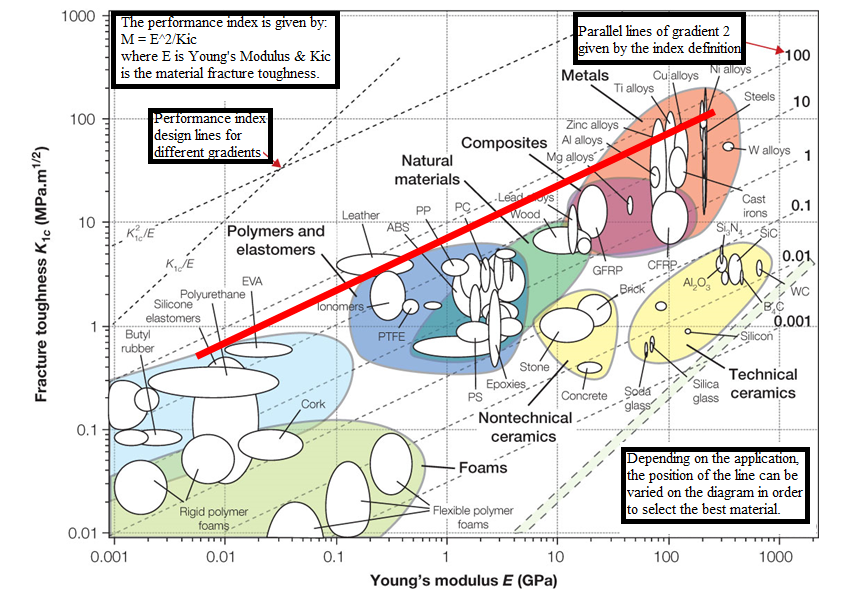
\includegraphics[width=13cm]{KicModulusAshby}
    \caption{Fracture Toughness vs. Young's Modulus \cite{MATPROPERTIESREF}}
    \label{young}
\end{figure}

\begin{figure}[hptb]
    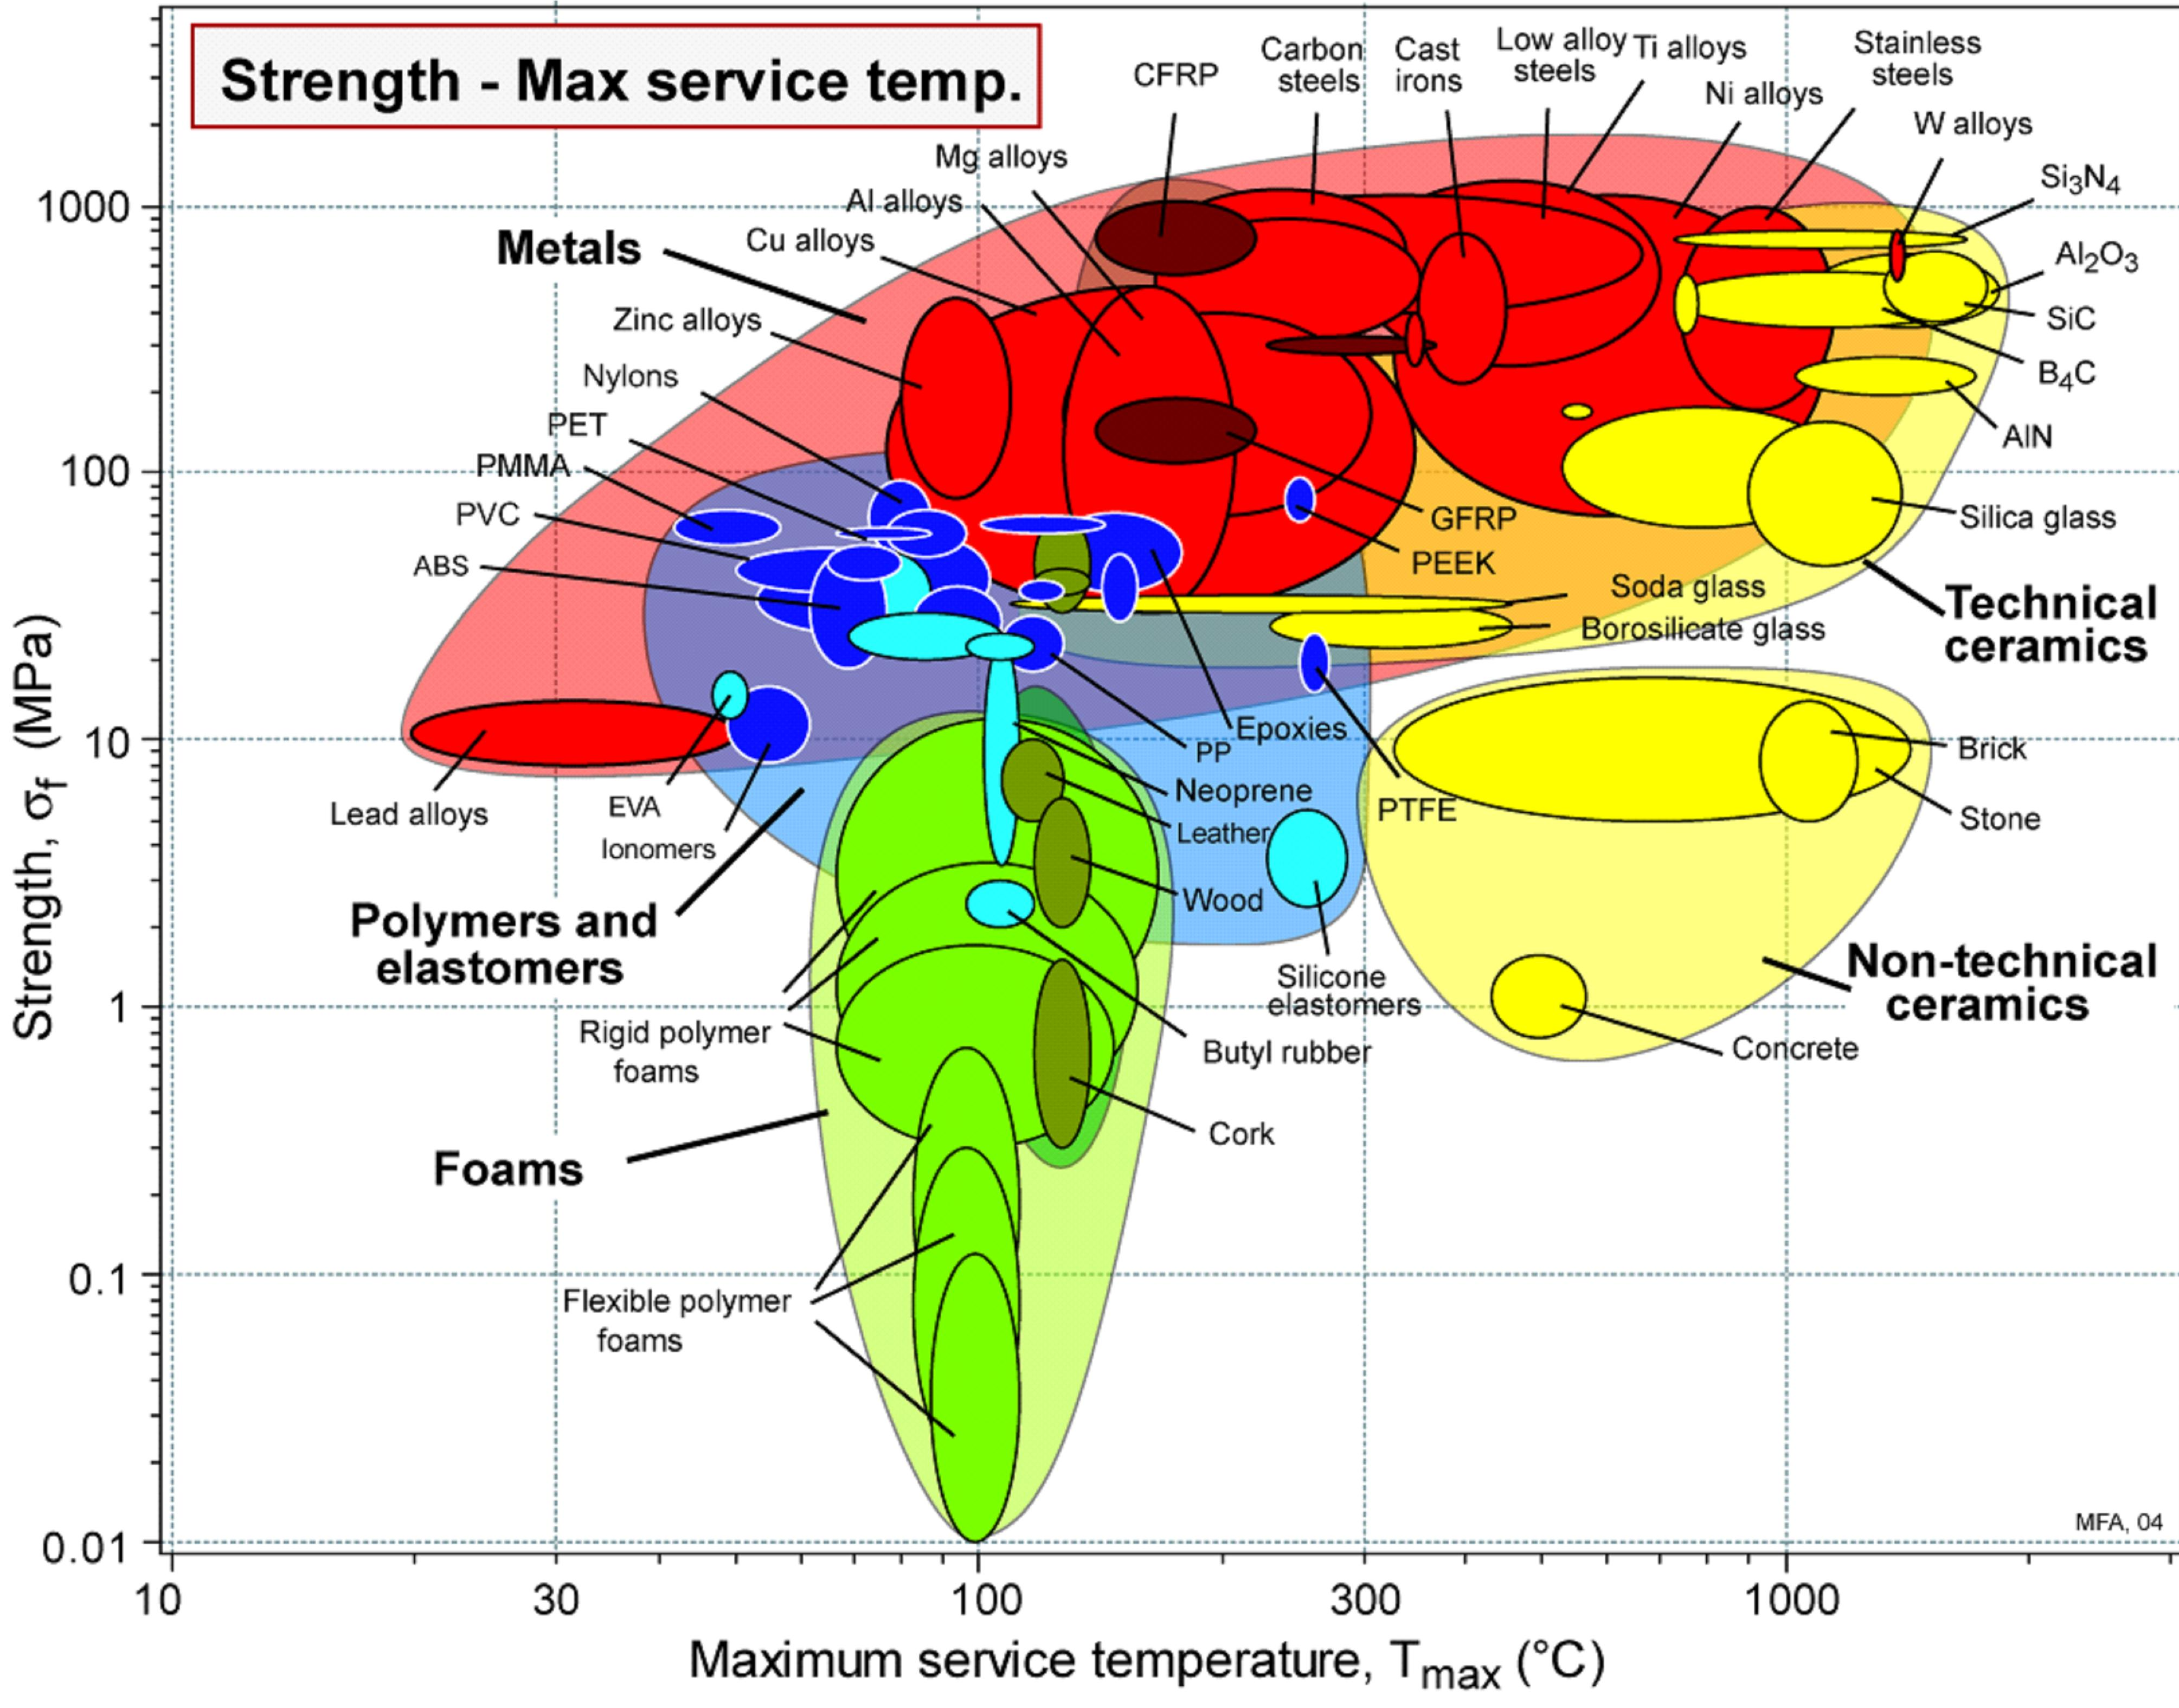
\includegraphics[width=11cm]{AshbyStrengthMaxTem.jpg}
    \caption{Strength vs. Maximum Service Temperature \cite{MATPROPERTIESREF}}
    \label{strength}
\end{figure}

\noindent Figure \ref{strength} plots the material strength against their maximum service temperature. The cruise speed has been considered to have a maximum of $25m/s$. At sea level, the speed of sound is approximately $340m/s$. This results in a Mach number less than 0.3; thus, the compressibility effects can be not taken into account. However, there will be motors and other electrical devices having different resistances, and therefore, energy will be lost under the form of heat. Further CFD will be performed in order to estimate the expected temperatures inside the UAV. \\

\noindent From the diagrams, ABS has a low fracture toughness and Young’s modulus compared to wood and carbon fibre reinforced polymers, the latter having the best performance in terms of stiffness and ability to plastically deform before fracture. In terms of Strength vs. Max. Service Temperature, ABS has a lower service temperature compared to wood, but a higher strength. Again, carbon fibre reinforced epoxy has the best performance, having a very high strength and a relatively higher service temperature. \\

\newpage
\begin{landscape}
\begin{center}
    \begin{tabular}{ | c | c | c | c | c | c |} 
    \hline
    \makecell{\textbf{ Material}} & \makecell{\textbf{Density} \\ $(kg/m^3)$} & \makecell{\textbf{Young's} \\ \textbf{Modulus} \\ $(GPa)$} & \makecell{\textbf{Tensile} \\ \textbf{Strength} \\ $(MPa)$} & \makecell{\textbf{Fracture} \\ \textbf{Toughness} \\ $(MPa.m^0.5)$} & \makecell{\textbf{Max. Service} \\ \textbf{$Temp.({\circ}C)$}}\\ 
    \hline
    \makecell{\textbf{Balsa wood}} & \makecell{160 - 300 } & \makecell{7.2 - 8.8} & \makecell{25 - 35} & 0.6 - 0.7 & 80 - 140\\ 
    \hline
    \makecell{\textbf{ABS}} & \makecell{1030 - 1040} & \makecell{1.4 - 3.1} & 2.34 & 2 - 3.67 & 60 - 75\\ 
    \hline
    \makecell{\textbf{All Purposes} \\ \textbf{PLA}}& \makecell{1240 - 1270} & \makecell{3.3 - 3.6} & 47 - 60 & 3.34 - 4.79 & 45 - 55 \\ 
    \hline
    \makecell{\textbf{Carbon fibre} \\ \textbf{reinforced} \\ \textbf{Epoxy - 50\%} \\ \textbf{fibres}} & \makecell{1600} & \makecell{55.1 - 60.6} & 245 - 278 & 4.8 - 5.8 & 140 - 220 \\ 
    \hline
    \end{tabular}
    \captionof{table}{UAV Structural Sub-assemblies}
    \label{prop}
\end{center}
\end{landscape}

\paragraph{B. Weight Calculations}
Typical full-scale aircraft weight calculations are based on the empty, fuel, crew and passengers weights. In the case of a small-scale UAV, as the propulsion system is using an electrical motor, those weights are practically equal to zero. Thus, a different approach was required to estimate a maximum take-off weight that shall be used used in all the preliminary design calculations. The typical method used in small-scale aircraft modelling is to consider the mass of the avionics and multiply it by a factor of 2-3 in order to estimate the overall mass of the UAV. \\ 

\noindent The estimated mass of the avionics is expressed in the table below. However, the motor has not yet been selected yet. Thus, our mass estimations were based on the average mass experienced by the models designed in previous years as part o this module. Therefore, the maximum take-off mass used in all the preliminary design calculations is $3kg$. \\

\begin{longtable}{ | c | c | c | c |} 
    \hline
    \makecell{\textbf{Components}} & \makecell{\textbf{Dimensions} \\ \textbf{($mm x mm x mm$)}} & \textbf{Quantity} & \makecell{\textbf{Weight} \\ \textbf{($g$)}}\\ 
    \hline
    \endhead

    \hline
    \textbf{PIXHAWK} & \makecell{81.5 x 50 x 15.5} & 1 & 38\\ 
    \hline
    \textbf{Camera} & \makecell{45 x 35 x 15} & 1 & 10\\ 
    \hline
    \makecell{\textbf{Official OSD} \\ \textbf{Board} \\ \textbf{PIXHAWK}} & \makecell{17.8 x 43.2 x 7.6} & 1 & 17 \\ 
    \hline
    \makecell{\textbf{Transmitter for} \\ \textbf{FUTABA} \\ \textbf{+} \\ \textbf{ENCODER}} & \makecell{43 X 25 X 9} & 1 & 7.8 \\ 
    \hline
    \textbf{GPS + Compass} & \makecell{60mm diameter} & 1 & 32\\ 
    \hline
    \textbf{APM Module} & \makecell{30 x 30 x 5} & 1 & 18 \\ 
    \hline
    \textbf{Video Transmitter} & \makecell{28.5 x 20 x 8} & 1 & 6.8\\ 
    \hline 
    \textbf{Telemetry Kit} & \makecell{50 x 20 x 10} & 1 & 57 \\ 
    \hline
    \textbf{Battery} & \makecell{137 x 44 x 19} & 1 & 250\\ 
    \hline
    \makecell{\textbf{Battery Monitor \textbackslash } \\ \textbf{Alarm 1-8S}} & - & 1 & 8.7 \\ 
    \hline
    \textbf{Tail Plane SERVOS} & 28 x 12 x 29 & 1 & 17 \\ 
    \hline
    \textbf{Flaps SERVOS} & 28 x 12 x 29 & 1 & 17 \\ 
    \hline
    \textbf{SERVOS Setup} & 28 x 12 x 29 & 1 & 17 \\ 
    \hline
    \textbf{ECS/Motor} & TBC & 1 & TBC \\ 
    \hline
    \textbf{I2C Board} & 50 x 20 x 10 & 1 & 10\\ 
    \hline
    \textbf{LED + USB Module} & 76 x 51 x 3 & 1 & 9 \\ 
    \hline
    \textbf{Airspeed Sensor} & 120 x 78 x 16 & 1 & 15 \\ 
    \hline
    \makecell{\textbf{Video Transmitter} \\ \textbf{Battery}} & 72 x 36 x 19 & 1 & 25 \\ 
    \hline
    \textbf{Total} & - & - & 546.3\\ 
    \hline
    \caption{Avionics Weight}
\end{longtable}

\paragraph{C. Centre of Mass} For the best performance of an aircraft, the centre of mass of the entire body should lie around 25\% of the chord length, from the wing's leading edge. In Figure \ref{masscentre}, it is shown the finalised model with the blue circles centred over where SolidWorks pin points the body’s centre of mass. This centre of mass is situated at about 78\% of the chord length, from the wings leading edge - way behind where it should be to achieve the best performance. However, this is acceptable for the final model, as the hollow fuselage will carry the components inside, enabling the team members be fixed down the avionics in different positions to achieve the optimum centre of mass.

\begin{figure}[h!]
    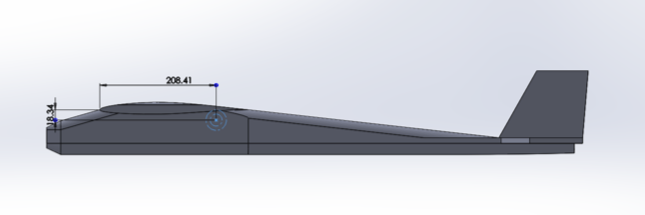
\includegraphics{centremass.png}
    \caption{Location of the Centre of Mass}
    \label{masscentre}
\end{figure}

\paragraph{D. Control Surfaces} The primary control surfaces on an aircraft are the Ailerons (roll control), Elevators (pitch control) and the Rudder (Yaw control); these need to be correctly designed in order to ensure that a sufficient amount of force is provided onto the surface in order to change direction of the aircraft. To appropriately design the control surfaces, they were modeled in ANSYS Fluent; the aircraft was moddeled in steady level flight in order to analyse the applied forces and decide upon the correct sizing of all control surfaces. \\

\noindent \textbf{1. Ailerons} \\

\noindent The sizing of the ailerons is an important part of the preliminary design as it allows the UAV to be designed and modelled appropriately; it also indicates the optimum size for servo motors needed to ensure sufficient applied force to change direction. An initial sizing for the ailerons is calculated using an online resource \cite{AILERONREF}, which says \emph{"ailerons typically extend from about 50\% to about 90\% of the span"}; with this advise, the chosen size of the ailerons would be a medium at 70\% of the span, meaning about $1.05m$. Translating this into two ailerons, this would give two $500mm$ ailerons. Then using Figure \ref{fig:aileron}, the 70\% value translates to a ratio of 0.15 aileron chord over wing chord. This is equivalent to the aileron chord being 40mm. Using this approach, the ailerons would be sized $500mm x 40mm$, much larger than the initial thoughts in the first sketch.

\begin{figure}[H]
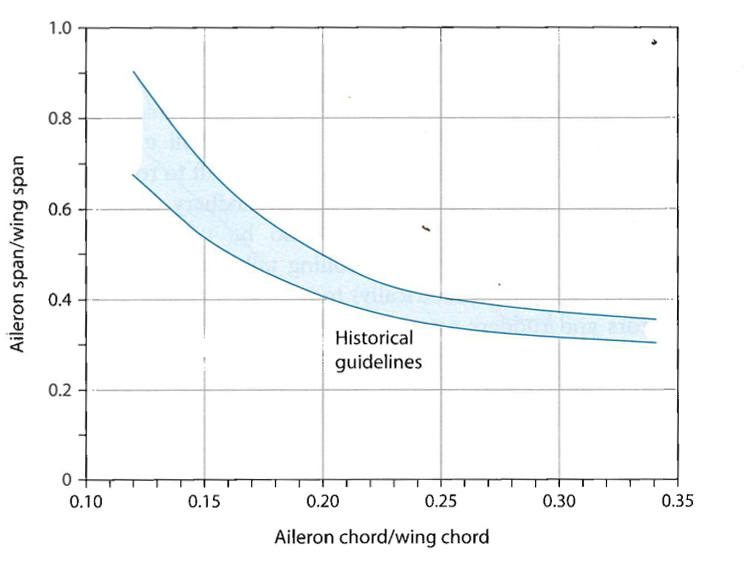
\includegraphics[width=13cm, scale=1]{aileron.png}
\caption{Aileron Guidelines \cite{AILERONREF}}
\label{fig:aileron}
\end{figure}

\noindent To ensure this approach gave appropriate results, the ailerons were modelled in ANSYS Fluent to test the forces applied. The NACA 65212 was modelled with the new sized aileron and tested at $25ms{{^-}^1}$ in steady level flight, with the aileron at 50 degrees (the maximum angle it should need to experience). \\

\noindent The results that were obtained showed a force of $27.7N$ over the face of the aileron, in that instantaneous moment at 50 degrees, travelling at $25ms{{^-}^1}$. This is a large force and shows plenty of excess if the aircraft needs to pull extreme manouveres. However, the purpose is to climb, cruise and descend at comfortable limits. So, this aileron sizing will be more than enough. 

\begin{figure}[H]
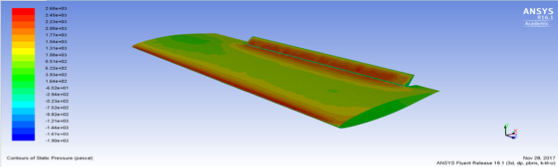
\includegraphics[width=18cm, scale=1]{aileroncfd.png}
\caption{Static Pressure Applied to Aileron at $25m/s$}
\label{fig:aileroncfd}
\end{figure}

\noindent Figure \ref{fig:aileroncfd} shows the static pressure applied to the aileron, including the points of concentrated force which are important to know as they give an estimate of where to reinforce the aircraft when constructing it. \\

\noindent With the ailerons tested with sufficent results, the rest of the method is adopted to chose the size of the elevators and rudder. \\

\noindent \textbf{2. Elevators} \\
\noindent Figure \ref{fig:elevatorandrudder} shows that the closest aircraft to the UAV is a 'GA[General Aviation] Single'; the calculations for elevator chord are at: \\

\begin{equation} \label{eq}
\frac{C_e}{C}=0.45
\end{equation}

\begin{figure}[h!]
    \includegraphics[width=12cm, scale=1]{elevatorandrudder.png}
    \caption{Control Surface Sizing Guidelines \cite{AILERONREF}}
    \label{fig:elevatorandrudder}
\end{figure}

\noindent \textbf{3. Rudder} \\
\noindent Using Figure \ref{fig:elevatorandrudder} and the same technique adopted in elevator calculations, the calculations for the rudder chord are at: \\

\begin{equation} \label{eq}
\frac{C_r}{C}=0.4
\end{equation}

\paragraph{E. Dimensions and Geometries} The engineering drawings below show the main sub-assemblies (wings, fuselage and tail) defined in terms of shape, dimensions and positioning. \\

\noindent All the geometries and dimensions defined in the drawings are based on the previous theoretical calculations that have been validated by the analysis performed in both XFOIL and Ansys Fluent. \\

\noindent Further changes in the dimensions of the fuselage will be considered in order to accomodate all the avionics without restricting them in any possible way. \\

\begin{figure}[h!]
    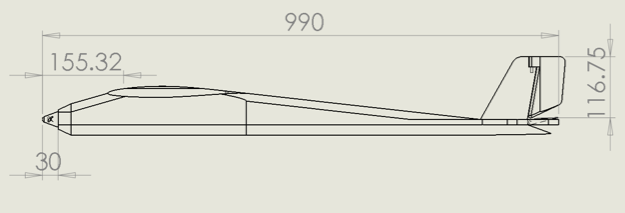
\includegraphics[width=14.5cm, scale=1]{drawing2.png}
\end{figure}

\begin{figure}[h!]
    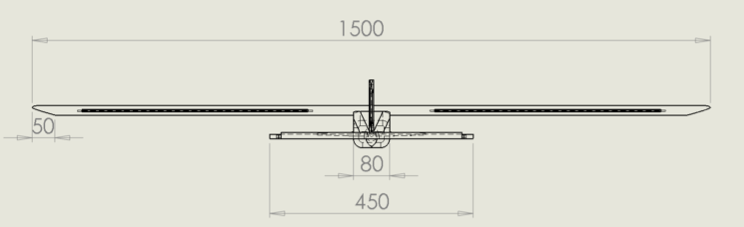
\includegraphics[width=14.5cm, scale=1]{drawing3.png}
\end{figure}

\begin{figure}[h!]
    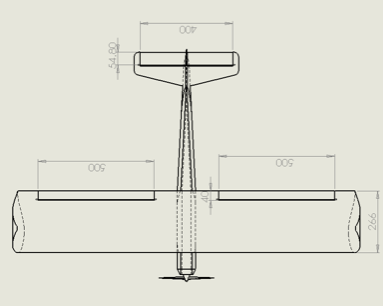
\includegraphics[width=14.5cm, scale=1]{drawing1.png}
    \caption{Engineering Drawings - Dimensions and Position}
\end{figure}

\newpage

\subsubsection{Ground Station and Communication}

\paragraph{Ground Control} To fly the UAV from the ground, the team has been assigned a Futaba T6K Proportional R/C system, which is a versatile remote controller designed for model plane hobbyists. The first course of action that was taken regarding the controller was to find a way for it to communicate with the UAV which will be done via a FUTABA R3006SB 6 CHANNEL 2.4GHZ T-FHSS S-BUS RECEIVER. This receiver is also manufactured by Futaba and designed for the considered controller and it is thought to be, most likely, the safest and most reliable option. The next step is to map the various servos on the UAV to their corresponding controls on the remote controller. Detailed instructions on how to do this are found in the manual for the controller, however, as manufacturing o the UAV has not yet started, it would be beyond the remit for a preliminary design report to list them here. \\

\noindent With regards to the ground station, the team decided to follow the same design principles used in the UAV mechanical design, simplicity and usability. The design based upon a briefcase style equipment case, filled with foam to protect the equipment. There would be a cut out on the bottom of the case to house the laptop, and similar cut outs on the lid, in which the video and telemetry receivers and their associated wirings could be mounted. These would either be held in place with glue or Velcro, as this would allow for the repositioning of the equipment if needed. This setup would make the ground station much more functional than just the components on their own, by adding extra protection and facilitating transportation. The setup time would also be improved, being closely reduced to zero, by having all items connected at once, rather than plugging them in each time. \\

\noindent In order for the pilot to be able to fly via the ground station video feed, there would have to be a very low latency in the system. For this reason, an analogue transmission was chosen over a digital system as, or the latter case, it takes a relatively long time for the system to process the digital signal. In addition to this, if the UAV was to fly out of range, with the analogue system, the picture would degrade gradually, acting as a warning for the pilot, so they could turn around before the signal was lost completely. In a digital system, the picture would become “jumpy” and then drop out completely, which would make recovery of the picture very difficult. \\

\noindent In order to actually get the video from the UAV onto the laptop screen, on the ground, the team is using a ProDVR Mini Video/Audio Recorder in conjunction with an EasyCap USB Video Capture device. The proDVR receives the signal and then transforms it into an AV signal that the EasyCap can read. The EasyCap then plugs into the laptop via a USB port and the video can be shown on screen in real time with the use of free EasyCap software. This solution should be very simple to implement as both of these components draw their power from the laptop; so there is no need for an external power source. \\

\noindent The telemetry data is slightly simpler; a $500mW$ Unmanned 3DR Telemetry Kit V2 ($433MHz$) kit was bought. This kit contains a two 433MHz transceivers – one for the UAV and one for the ground station – which will allow communication between the two. At $500mW$, this kit is as powerful as it can legally be (SEE SAFETY AND LAW) and should provide the UAV with an excellent range. As with the video receivers, this does not need an external power source for the ground station, resulting in the simplicity of the design. \\

\noindent The software being used for the telemetry data and course plotting on the ground station is ‘Mission Planner’ which is a free software, easily available on the web and comaptible with the Pixhawk autopilot installed on the UAV. It was chosen as it is very intuitive to use and mission planner makes it very easy to install the necessary firmware onto the Pixhawk; this process is as simple as plugging the Pixhawk into the laptop, waiting for the two to connect, following the prompts on screen and then disconnecting and reconnecting the Pixhawk again. Figure \ref{mission} shows the interface used with this software, all of the telemetry data being shown on the left, whilst the positioning of the UAV on the right. One important feature of the mission planner software is its ability to set waypoints on this map that the UAV can then fly to automatically. \\

\begin{figure}[hptb]
    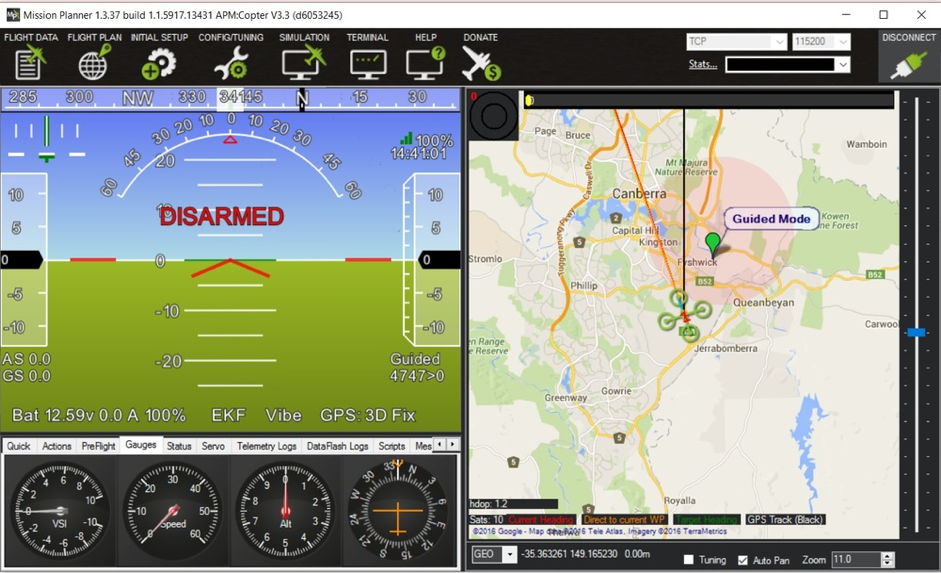
\includegraphics[width=13cm]{mission_planner.png}
    \caption{Mission Planner User Interface}
    \label{mission}
\end{figure}

\noindent One idea the team has explored in order to impart functionality to the UAV is having two cameras – one mounted in line with the propeller to provide a first-person view and a second camera mounted in the lower part of the fuselage of the aircraft to provide a view of the ground. The first-person view would allow the pilot to control the UAV, even when they do not have line of sight with it via the video feed, on the ground station. In addition to this, the ground facing camera would allow for ‘reconnaissance’ work at the same time. Having two cameras would obviously take up more space, weight and power, but they are relatively small; thus, these would be negligible in reality. Another potential disadvantage would be the transmitting and receiving of two video streams at the same time. The way around this is to make sure that the transmitters that has been selected are able to transmit and broadcast on different channels, as the two streams would interfere with each other; however, in reality, most camera/transmitter products have this functionality built in. \\

\noindent Unfortunately, whilst the team agreed that having two cameras could bring a significant increase in the functionality of the UAV, the idea has been put on pending due to budgetary requirements; provisions have been made in order to allow the installation of a second camera and if the UAV comes in under budget, a second camera will be integrated into the design. \\

\subsubsection{Control - Autopilot\textbackslash Autostabilisation}

\noindent In tackling this part of the design, the various possibilities that the chosen autopilot unit can offer have been evaluated.  The chosen autopilot is the Unmanned Pixhawk autopilot unit. This particular model of the autopilot has been chosen as it is a cheaper version of the 3DR Pixhawk unit and at the same time it offers all the necessary connectivity and components necessary for our design. \cite{CONTROL1} The main firmware used for our mission will be Pixhawk firmware, uploaded from "Mission Planner". This is the firmware that will be loaded onto our autopilot unit and it will provide all the necessary functionalities that are going to be needed for our flight mission. For the ground control station, the software that will be used is "Mission Planner". This is the best software available for windows operating systems and it's compatible with the Pixhawk firmware and various FPV systems(First-person view; for more details refer to Section3.3.5). Both softwares are available for free download from the Ardupilot's website.\cite{CONTROL2} \\

\noindent Thinking about the level of autonomy that the UAV has to have, the possibilities taken into consideration were various. The autopilot offers a range of flight modes, going from a completely autonomous flight mode to a completely manual flight mode. \\

\noindent Of the major flight modes, the ones taken into consideration are: the "MANUAL mode", "AUTO mode", "Stabilize mode" and "FLY BY WIRE A". During the testing phase for all the servos, sensors and components functionalities, the manual mode would be used. This mode gives complete control over the UAV to the pilot through the FUTABA T6K controller. \cite{CONTROL3} \\

\noindent For the actual flight session, since the autopilot has a reliable and advanced autonomous mode, this will be used for most of the flight; the AUTO mode will be controlled through the use of "way-points" and "do commands". To start the "Auto" mode, a couple of important steps must be taken in advance. To enter the Autonomous mode, it is necessary to make sure that the motor has been armed, the various control surfaces checked and the autopilot tested. During this testing phase on the ground, the first mode to be used is the "Manual mode"; by using it, the control surfaces can be tested individually to make sure each component is properly responding. Once this process has been successfully completed, the next stage is to enter the "Stabilize mode"; in this mode, it is possible to arm the motor. Leaving the "ARMING\_REQUIRE", "ARMING\_CHECK" and "ARMINF\_RUDDER" options as default on the Pixhawk firmware, the motor can be armed by holding the rudder stick fully to the right for 2 seconds, while the GPS can be armed, by pressing the arming button on the "Mission planner" ground station. After that, it is necessary to wait 30 seconds to make sure the GPS has locked the position.\cite{CONTROL4} \\

\noindent Another important step that has to be done in this mode is to test the autopilot. This can be done, by staying on "Stabilize mode" and manually move the UAV in a pitching and rolling position. If the autopilot is working correctly, the ailerons and tail plane surfaces should move to produce an opposite moment, stabilizing the aircraft (this is due to the fact that the UAV is in its "stabilized" mode). Now that the motor is armed, control surfaces are checked and autopilot tested, the last step is to switch to Autonomous mode, making sure that the GPS is locked and finally prepare for the launch. \\

\noindent In the autonomous mode, the most important step is to set your commands and waypoints. By setting waypoints on Mission planner, the software can communicate these points to the Pixhawk through the telemetry antenna. Once the data reaches the UAV, this will, relying on its GPS unit, make sure to go to these points and follow the altitude, coordinates and commands given at each "waypoint". \cite{CONTROL3} \\

\noindent For each "waypoint", it is possible to force the UAV to execute certain actions from a long list of commands. These include: loiter (i.e. circle around, maintaining a certain altitude), cruise, return to launch coordinates, etc \ldots \cite{CONTROL3} \\

\noindent Usually, for most of the way points, the command is generally just "WAYPOINT". By using this command, the UAV will simply go through that point, at the specified altitude and not do any particular action. The Pixhawk will make sure to adjust to any sudden change in heading altitude and position, by autonomously acting on the control surfaces and throttle. \cite{CONTROL5} Using these commands and the "way-points", it is possible to create different paths and execute various flight manoeuvres. \\

\noindent The only two parts of the flight where there are some slight complications are the take-off and landing phases. Ideally, the best option would be to have a fully autonomous take-off and landing. These can be achieved by inputting, on the first and last "way point", the commands "TAKE-OFF" and "LAND". In addition, a set of values has to be specified for each of the two cases. These values help the autopilot perform the correct take-off and landing procedures. The type of input values are dependent on the type of take-off chosen. \\

\noindent In our case, by requirement, the take-off has to be a conventional/runway take-off. The design chosen for the landing gear is a tricycle landing gear configuration. Therefore during take-off, the values to be specified in the Mission Planner/Pixhawk software are "THR\_MAX", "TKOFF\_ROTATE\_SPD", "TKOFF\_THR\_SLEW" and "TECS\_PITCH\_MAX". The first value is the maximum thrust allowed and this shall be used during this phase. The second value is the speed at which the UAV will start to pitch up, starting the take-off; this should be $2m/s$ above the stall speed or more. The third one represents the percentage/second at which the throttle rumps up during take-off (throttle slew rate) - a value between 20\% to 30\% /second should be a good enough value. Finally, the last value controls the maximum pitch used when climbing during take-off; usually a value around 20 degrees is a fairly safe angle of climb. \cite{CONTROL6} \\

\noindent For the landing, the command used is "LAND". This command requires a few set values, to be able to properly work. The first value determines the time in seconds before the UAV has contact with the ground, at which the aircraft needs to start flaring to make a slow and smooth landing(LAND\_FLARE\_SEC). Alternatively, a setting for the altitude can be used instead of time, to control the height at which the aircraft should start the flare manoeuvre(LAND\_FLARE\_ALT). Another important factor is the distance and altitude between the last way point and the landing point; this has to be decided to control the glide slope and avoid steep gliding slopes. Landing airspeed (TECS\_LAND\_ARSPD) and the priority between the landing speed and gliding angle (TECS\_LAND\_SPDWGT) need to be set as well. \cite{CONTROL7} \\

\noindent To get these parameters, it is feasible in theory, and most of the values can be found by applying theoretical methods. The main issue is that, these values are also strongly dependent on the type of fuselage/wings used and it requires fine tuning and a series of tests to make sure that everything behaves correctly. In our case, this is not possible as there is no way to practically test our UAV beforehand. Therefore, another approach that could be considered is to rely on the semi-manual "Fly by wire A" ("FBWA": roll and pitch are held) flight mode; this mode can be used during both landing and take-off. \\

\noindent As this is only the initial stage of the design, both approaches are still being considered. The choice of not completely discard the autonomous mode is also reinforced by the fact that it could also be possible to set take-off and landing in auto mode and override the commands (taking manual command), if the aircraft happens to go out of the indicated parameters. \\

\noindent This can be easily done by switching flight modes and simply going back to a stabilized or fly by wire mode. The Futaba T6K allows us to have up to four different flight modes and therefore, at this point by leaving one of the four on autonomous mode, it would still be possible to go back and, at any time, by using the Futaba controller switch, change to a different mode and proceed to land or take control of the aircraft, either utilising the "Stabilized mode" or the "FBWA" (fly by wire), keeping the plane stable during the mission. \cite{CONTROL8} To conclude, the approach taken is to have one of the Flight modes on "Autonomous" with "way points" deciding the path for our mission. Take-off in autonomous flight should not be too risky to design. On the other hand, the landing, given the amount of data and the number of parameters that need fine tuning and testing, might be done using the safer "FBWA" mode. \\

\noindent The last two channels are left for "Stabilized mode" and "Manual mode" in case the aircraft needs to be quickly recovered from a dangerous situation during the flight. \\

\subsubsection{Sensors, Actuators and Communicators}

\noindent The configuration used for the UAV is based on the main component, which, in this case, is the Pixhawk autopilot. This, as explained in the Section3.3.4, provides numerous functionalities and control options for our aircraft; but in order to be able to make use of all these functionalities, a number of components have to inserted in our configuration and coupled with the Pixhawk. \\

\noindent In this case, the battery that is going to be used is a LiPo (Lithium polymer) $7.4V$, $5000mAh$ battery. The Pixhawk controller needs a stable $5.37V$ and $2.25Amp$ power supply. It would be totally unsafe and impossible to control, to try to provide this power, directly from the battery. An APM Power Module is going to be connected between the LiPo battery and the Pixhawk providing it, with a stable supply of power (APM specifications : $5.3V$ and $3A$ max output). By connecting the APM to the Pixhawk, not only is the autopilot going to be powered, but it's also going to be possible to monitor the battery, allow the firmware to compensate for interferences on the compass unit and in the case the voltage becomes too low, it would be possible to automatically start a "Return to Launch" function to bring the aircraft back to the base. \cite{SENSOR1} \\

\noindent Another really important component in our configuration is the Receiver, this is the unit that is going to allow us to communicate with the Pixhawk via the Futaba T6K controller. Thanks to the power module plugged into the Pixhawk, the receiver is going to be directly powered by the Pixhawk/power module. Therefore, all we need to do is plug the receiver into the Pixhawk. \\

\noindent In choosing our receiver, the main 3 options that were evaluated were: "Pulse Width Modulation" (PWM) receivers, "Pulse Position Modulation" (PPM) receivers and "Serial Bus" (S.Bus) receivers. Each one of these 3 receivers offers advantages and disadvantages, for example the PWM receiver, while being the most common and the cheapest of the three, it also has a lot of wires and the signal outputted cannot be read by the Pixhawk, thus it would need a PWM to PPM encoder to convert the signal to PPM before it could be read by the autopilot. The PPM allows for up to 8 channels to be transmitted through a single wire, the downside is that these channels are transmitted one at the time, making it a slightly more inaccurate. Finally, S.BUS, this is the receiver chosen for our design. This is because through a single wire the S.Bus can transmit up to 18 channels, the only issue with this receiver is that it's not compatible with many flight controllers, but this does not apply to our case, since the Futaba T6K can transmit to the S.BUS receiver and this can be directly connected to our Pixhawk, so there are no compatibility problems. The S.BUS receives 6 channels at $2.4GHz$ and the same frequency and number of channels is transmitted by the Futaba T6K. This is the perfect frequency for our design; our main interest in transmitting the signal is the range (our mission may take the aircraft at long distances from the ground base), at the same time the speed at which the signal is transmitted is not as important, so there is no need to have a higher transmission frequency. The commands are mostly autonomous and even in case of signal transmission from the controller, the time scale of the "delay" is basically negligible, the UAV will not perform any high velocity, acrobatic manoeuvres. This coupled with the fact that the controller, already has a default transmission frequency of $2.4GHz$, makes of the Futaba $2.4Ghz$, the perfect receiver for our UAV. \cite{SENSOR2}\cite{SENSOR3} \\

\noindent To transmit the position of the UAV, battery voltage and other data to the ground base, a telemetry radio unit has to be utilized. One of the two antennas, in the telemetry kit, has to be connected to the Pixhawk and it will be directly powered by the Power Module, so there is no need for an external power supply. The other antenna is to be connected to the ground station (Refer to Ground Station section). The frequency of transmission is 433 MHz, this is a relatively low frequency and therefore the signal has a pretty good range. The power parameter is 500 mW which is the maximum legal power parameter for radio transmission in UK. \cite{SENSOR3} \cite{SENSOR4} \\

\noindent To have an accurate GPS signal, a GPS + compass unit is used, this is powered by the APM/LiPo battery combination and it's directly connected to the Pixhawk. \cite{SENSOR5} \\

\noindent A buzzer and a safety switch are both included with the Pixhawk and have to be connected to the autopilot, these components are required for safety purposes. \cite{SENSOR5} For what regards the motor (Refer to the Propulsion section) and the servos, these cannot be powered by the power module. For these components, an ESC (electronic speed controller) module is necessary. Once the ESC has been connected to the power module and to the Pixhawk, it's possible to connect the motor (with propeller) to the ESC. By doing this we are able (after the calibration of the ESC) to control the motor speed through the autopilot. The ESC, once connected to the Pixhawk, will also allow us to simply plug all our servos into the Pixhawk and be able to power them using the ESC and control them using the Pixhawk. \cite{SENSOR6} \cite{SENSOR7} ESC Board is chosen after adding 10\%-20\% more to the amp rating of the motor and making sure that motor and ESC can handle the same amount of battery cells, in our case, 2. The ideal ESC should also have a BEC ( Battery Eliminating Circuit) incorporated, to allow us not only to control the speed of the motor, but to also provide a regular $5V$  supply to power our components (because our battery is $7.4V$). This could be for the FPV system or for the motor itself (this applies to both fixed wings and multirotors). \cite{SENSOR11}\\

\noindent The servos chosen are to be able to exert a force of at least $25N$ force and do it in the smallest possible time, due to budget limitation and to stay true to these requirements, the chosen servos for ailerons, rudder and elevators are the Finwing $17g$ Servo. These servos provide $2.5kg/cm$ torque and $0.10sec/60^{cirq}$ speed at 6 volts and  these are the servos usually used for aircrafts with a gross weight below $4.5kg$, which also matches our case. \cite{SENSOR8} \cite{SENSOR9} For our design, a live video feed is also required, this is provided through the use of an FPV system. The system consists in an FPV camera, a minim OSD board and an secondary battery to power the FPV system. The battery is going to be a $1000mAh$, 11.1 V 3S battery connected to a XT60 plug, this is going to be used to power a $5.8GHz$ 40Ch $200mW$ (voltage range $7 - 24V$) video transmitter and an FPV Sony camera (HS1177, operational voltage range: $5 - 22V$), connected to an OSD V 1.1 minim board. This board takes the telemetry data from the Pixhawk autopilot and shows it over the live video feed coming to the ground base. (For schematic of the FPV system refer to Figure \ref{fig:FPV system}) \cite{SENSOR10} \\

\begin{figure}[h]
    \centering
    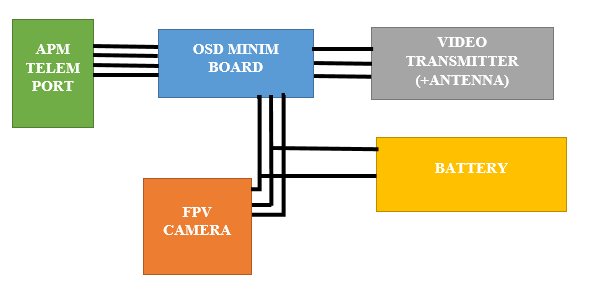
\includegraphics[width=0.70\linewidth]{Diagram.png}
    \caption{FPV system scheme}
    \label{fig:FPV system}
\end{figure}

\begin{figure}[h!]
    \centering
    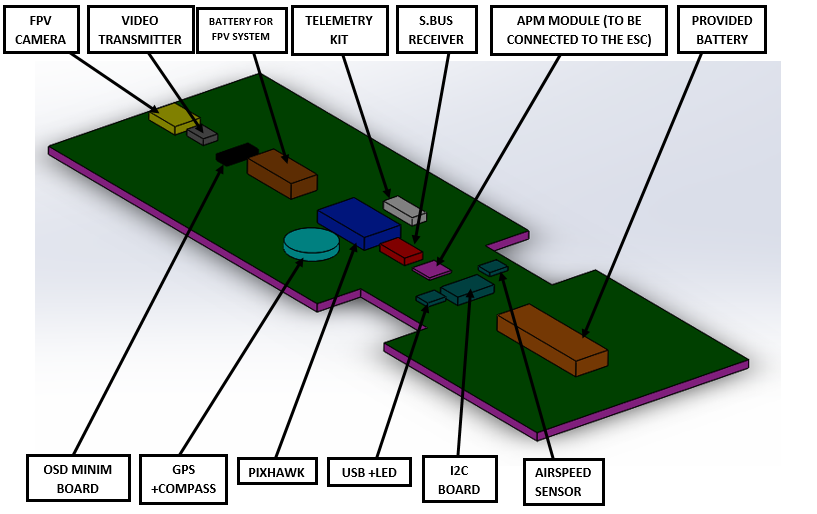
\includegraphics[width=1\linewidth]{components.png}
    \caption{Avionics components scheme}
    \label{fig:Avionics}
\end{figure}

\noindent The frequency used to transmit the video signal is $5.8GHz$, this is used in most FPV systems as the go to transmission frequency. This high transmission frequency is explained by the fact that, this time, the signal is quite important to us, because it carries the video and it has to be as clear as possible, therefore choosing a higher frequency (higher bandwidth) is our best option to have a clear and not delayed video feed.\cite{SENSOR11} \\

\noindent The last components to be inserted into our configuration are optional and they are the External USB port and airspeed sensor, both connected to the I2C splitter board, and this is connected to the Pixhawk powered by the Power module/5000mAh LiPo battery. These are components can be added at a later stage, assuming the budget permits it.\cite{SENSOR5} \\

\begin{figure}[h!]
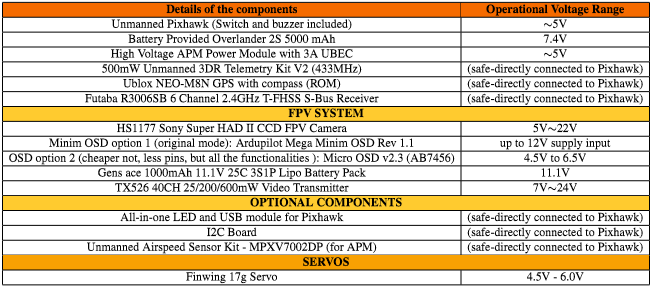
\includegraphics[width=18cm, scale=1]{Hamzatable.png}
\caption{Avionics Components and Their Voltages}
\end{figure}

\section{Conlusions Upon the Preliminary Design}

\textbf{A. Avionics - Control, Ground Station \& Actuators}\\
\noindent The final design is going to include a solution that makes full use of the capabilities of the Futaba controller. Using all 4 of the flight modes, it will be possible to have one fully autonomous mode, in which   through theoretical calculations, it will be possible to set all the parameters, for auto take-off and landing. At the same time, in order not to incur in any serious flight control problem, 2 of the 4 channels will be equipped with a semi manual mode ("Stabilize" and "Fly By Wire A"), which will make possible to take off and land while being assisted by the autopilot. The team's plan is to keep the cruise and flight path at altitude fully autonomous (using "Way points"); the 4th mode is going to be left on fully manual, in case of complete break down of the autopilot, or just simply to manually test the different components on the ground.\\

\noindent For far as the sensors, communication and actuators are concerned, most of the components are ready to be ordered and hopefully soon enough, the components will be available to start testing/programming. Before this can happen, all that is left to do is to finalize the last details and make a final check of compatibility/voltage range between components. Once this is all done, it will be possible to start working with the sensors, making the necessary adjustment to ensure that the hardware and software of the control system is well implemented. As per what regards the type of components that will be used, these have been amply described in the relative sections; now the configurations and wirings has to be analysed in order to prepare for the next step. On a last note, the only board that has to be yet decided upon is the ESC, and while the method to make the decision has already been decided upon and described above, the motor on which this is based, has not yet been fully assessed. This is not a big issue as the first part of the design will focus on creating a stable, radio and video signal between ground station and Pixhawk/UAV, as well as between the Futaba controller and the Pixhawk. Once this will be done, the process can go into its next stage. \\

\noindent \textbf{B. Materials \& Structure}\\
\noindent The main options in terms of the materials are carbon fibre, ABS or PLA plastics and balsa wood. A mixture of these materials was preferred in order to efficiently use the available resources in such a way that stiffness, toughness and hardness could be provided in key areas, such as wings, tails and fuselage. 3D printed plastic is considered as a modality of producing intricate shapes, for a low weight and relatively acceptable weight. Carbon fibre shall be used in areas where increased strength is required due to loadings (i.e. wings and tail plane), while wood can be a reliable source for multiple iterations in design, perfect for testing shapes, geometries and joints. Various joining methods are considered, from nuts and bolts, to glue or tight fittings. Future plans in terms of structure includes producing individual drawings for each component and order material for a first design iteration. \\

\noindent \textbf{Aerodynamics}\\
\noindent Design features have been imparted on the UAV, starting from the design concepts that mimicked similar sized and purposed trainer aircrafts. From there, theoretical calculations were used to refine the aircraft’s sizing, aerofoil design and aircraft’s performance parameters. This has then been analytically backed up by using both XFOIL and Ansys FLUENT, in order to get an understanding of how the airflow behaves and its effects on the flight of the UAV. The next stages for aerodynamic design would include creating a miniature model to test in a wind tunnel and making a virtual model on the Merlin simulators to further ensure the design’s quality. The Merlin simulators in particular would be very useful in determining the UAV’s behaviour under realistic flight conditions as everything from control surface sizing to the choice of the aerofoil could be assessed by their realistic performance. \\

\newpage

\begin{thebibliography}{9}
    
\bibitem{REFERENCE1}
Ofcom. (2017). Short Range Devices Information Sheet. [online] Available at: $https://www.ofcom.org.uk/spectrum/radio-spectrum-and-the-law/licence-exempt-radio-use/licence-exempt-devices/short-range-devices-information$ [Accessed 30 Nov. 2017].

\bibitem{REFERENCE2}
6 - Channel Digital Proportional R/C System Manual, Futaba

\bibitem{TRAINERREF}
Tjdmodels.com. (2017). TJD Models, RC and Plastic Model Shop near J2 of the M25, Kent. [online] Available at: $http://www.tjdmodels.com/$ [Accessed 30 Nov. 2017].

\bibitem{CESSNAREF}
Cessna.txtav.com. (2017). Cite a Website - Cite This For Me. [online] Available at: $http://cessna.txtav.com/-/media/cessna/files/piston/skyhawk/skyhawk_brochure.ashx$ [Accessed 30 Nov. 2017].

\bibitem{TAKEOFFREF}
Anon, (2017). [online] Available at: cite $http://www-mdp.eng.cam.ac.uk/web/library/enginfo/aerothermal_dvd_only/aero/perf/to/index.html$ [Accessed 30 Nov. 2017].

\bibitem{NASAREF}
Grc.nasa.gov. (2017). Shape Effects on Drag. [online] Available at: $https://www.grc.nasa.gov/www/k-12/airplane/shaped.html$ [Accessed 30 Nov. 2017].

\bibitem{AILERONREF}
P. Raymer, D. (2012). Aircraft Design: A Conceptual Approach. 5th ed. American Institute of Aeronautics and Astronautics Inc., pp.161-162.

\bibitem{ESCREF}
DroneTrest. (2017). What to consider when buying a ESC for your multirotor. [online] Available at: $http://www.dronetrest.com/t/what-to-consider-when-buying-a-esc-for-your-multirotor/1305$ [Accessed 30 Nov. 2017].

%broken
% \bibitem{BALSAREF}
% Hobbyking. (2017). Planes. [online] Available at: $https://hobbyking.com/en_us/planes.html?___store=en_us$ [Accessed 30 Nov. 2017].

\bibitem{BALSAREF}
Hobbyking. (2017). Planes. [online] Available at: $https://hobbyking.com/en_us/planes.html$ [Accessed 30 Nov. 2017].

\bibitem{COMPOSITEREF}
Hull, D. and W. Clyne, T. (1996). An Introduction to Composite MAterials. 2nd ed. Cambridge University Press.

\bibitem{MATPROPERTIESREF}
Jones, D. and F. Ashby, M. (2015). Engineering Materials 1: An Introduction to Properties, Applications and Design. 3rd ed. Elsevier.

\bibitem{TAILSIZEREF}
Ocw.mit.edu. (2017). Cite a Website - Cite This For Me. [online] Available at: $https://ocw.mit.edu/courses/aeronautics-and-astronautics/16-01-unified-engineering-i-ii-iii-iv-fall-2005-spring-2006/systems-labs-06/spl8.pdf$ [Accessed 30 Nov. 2017].

\bibitem{CONTROL1}
Kit, U. and Tech, U. (2017). Unmanned Pixhawk Autopilot Kit. [online] Unmanned Tech. Available at: $https://www.unmannedtechshop.co.uk/unmanned-pixhawk-autopilot-kit/$ [Accessed 30 Nov. 2017].

\bibitem{CONTROL2}
Anon, (2017). [online] Available at: $http://ardupilot.org/planner/docs/common-loading-rmware-onto-pixhawk.html$ [Accessed 30 Nov. 2017].

\bibitem{CONTROL3}
Anon, (2017). [online] Available at: $http://ardupilot.org/plane/docs/ ight-modes.html$ [Accessed 30 Nov. 2017].

\bibitem{CONTROL4}
Ardupilot.org. (2017). Arming Plane — Plane documentation. [online] Available at: $http://ardupilot.org/plane/docs/arming-your-plane.html$ [Accessed 30 Nov. 2017].

\bibitem{CONTROL5}
Anon, (2017). [online] Available at: $http://ardupilot.org/planner/docs/common-planning-a-mission-with-waypoints- and-events.html$ [Accessed 30 Nov. 2017].

\bibitem{CONTROL6}
Anon, (2017). [online] Available at: $http://ardupilot.org/plane/docs/automatic-takeo .html$ [Accessed 30 Nov. 2017].

\bibitem{CONTROL7}
Ardupilot.org. (2017). Automatic Landing — Plane documentation. [online] Available at: $http://ardupilot.org/plane/docs/automatic-landing.html$ [Accessed 30 Nov. 2017].

\bibitem{CONTROL8}
FutabaT-FHSS Air-2.4GHz-6K; Manual Folder-AER385

\bibitem{SENSOR1}
Ardupilot.org. (2017). Common Power Module — Plane documentation. [online] Available at: $http://ardupilot.org/plane/docs/common-3dr-power-module.html$ [Accessed 30 Nov. 2017].

\bibitem{SENSOR2}
Anon, (2017). [online] Available at:$ http://ardupilot.org/plane/docs/common-pixhawk-and-px4-compatible-rc-transmitte and-receiver-systems.html$ [Accessed 30 Nov. 2017].

\bibitem{SENSOR3}
Ardupilot.org. (2017). SiK Telemetry Radio — Plane documentation. [online] Available at: $http://ardupilot.org/plane/docs/common-sik-telemetry-radio.html$ [Accessed 30 Nov. 2017].

\bibitem{SENSOR4}
Anon, (2017). [online] Available at: $https://www.ofcom.org.uk/spectrum/radio-spectrum-and-the-law/licence-exempt- radio-use/licence-exempt-devices/short-range-devices-information$ [Accessed 30 Nov. 2017].

\bibitem{SENSOR5}
Ardupilot.org. (2017). Pixhawk Wiring Quick Start — Plane documentation. [online] Available at: $http://ardupilot.org/plane/docs/common-pixhawk-wiring-and-quick-start.html$ [Accessed 30 Nov. 2017].

\bibitem{SENSOR6}
Ardupilot.org. (2017). Powering the Pixhawk — Plane documentation. [online] Available at: $http://ardupilot.org/plane/docs/common-powering-the-pixhawk.html$ [Accessed 30 Nov. 2017].

\bibitem{SENSOR7}
Ardupilot.org. (2017). Servo — Plane documentation. [online] Available at: $http://ardupilot.org/plane/docs/common-servo.html$ [Accessed 30 Nov. 2017].

\bibitem{SENSOR8}
Anon, (2017). [online] Available at: $https://www.buildyourowndrone.co.uk/ nwing-17g-servo$ [Accessed 30 Nov. 2017].

\bibitem{SENSOR9}
Anon, (2017). [online] Available at: $https://www.buildyourowndrone.co.uk/ nwing-sabre-arf$ [Accessed 30 Nov. 2017].

\bibitem{SENSOR10}
Ardupilot.org. (2017). Minim OSD Quick Installation Guide — Copter documentation. [online] Available at: $http://ardupilot.org/copter/docs/common-minim-osd-quick-installation-guide.html$ [Accessed 30 Nov. 2017].

\bibitem{SENSOR11}
Anon, (2017). [online] Available at: $http://www.rcdronearena.com/2016/03/15/wi -fpv-vs-5-8ghz-fpv-vs-2-4ghz- fpv-explained/$ [Accessed 30 Nov. 2017].
    
\end{thebibliography}

\appendix

\section{Apendix: List of Symbols}

\begin{longtable}{| c | c | c | c | c |}
        \hline
        \textbf{Character} & \textbf{Name} & \makecell{\textbf{Associated} \\ \textbf{Value}} & \textbf{Units} & \textbf{Notes}\\
        \hline
        \endhead

        \hline
        $W_{avg}$ & Average Weight & 24.525 & $N$ & \makecell{This value is subject \\ to future changes. \\ This value is equal \\ to the overall \\ weight of the \\ UAV.} \\
        \hline
        WTO & \makecell{Maximum \\ Take-off \\ Weight} & 24.525 & N & \makecell{This value is equal to \\ the average weight.} \\
        \hline
        $V_{c}$ & Cruise Speed & 25 & $m/s$ & \makecell{It can be reffered \\ to as u.} \\
        \hline
        $V_{stall}$ & Stall speed & 11.55 & $m/s$ & \makecell{The stall speed has \\ been assumed 10 m/s \\ for the initial \\ airfoil design \\ selection.} \\
        \hline
        $V_{take\_off}$ & \makecell{Take-off \\ Speed} & 13.86 & $m/s$ & \\
        \hline
        T & Thurst & 3.98 & $N$ &  \\
        \hline
        $\rho_{0}$ & \makecell{Air Density \\ at Sea Level} & 1.225 & $kg/m^3$ & \makecell{As the altitude \\ range is limited \\ to 10-30 m above sea \\ level, the air density \\ can be assumed \\ constant.} \\
        \hline 
        $\mu$ & \makecell{Air viscosity} & $1.857*10_{-5}$ & $kg/(m*s)$ & \\
        \hline
        S & \makecell{Wing Surface \\ Area} &  & $m^2$ & \makecell{This value is subject \\ to future changes.} \\
        \hline
        b & Wing Span & 1 & $m$ & \makecell{Assumed 1 m based \\ on the design \\ requirement. This \\ Value is subject \\ to future changes.} \\
        \hline
        c & Mean Chord &  & $m$ & \makecell{Considering a \\ rectangular wing, \\ the chord does not \\ vary between the \\ tip and the root \\ of the wing. This \\ value is subject \\ to future changes.}\\
        \hline
        Re & \makecell{Reynolds \\ Number} &  & - & \makecell{It may have various\\ values.} \\
        \hline
        $C_{lideal}$ & \makecell{Ideal Lift \\ Coefficient} &  & - & \makecell{It may have various\\ values in the \\ analysis.} \\
        \hline
        $C_{lmax}$ & \makecell{Maximum Lift \\ Coefficient} &  & - & \makecell{It may have various\\ values in the\\ analysis.} \\
        \hline
        \caption{Symbols Table}
\end{longtable}    

\section{Apendix Materials and Aerodynamic Design} 

\noindent \textbf{A} Figure \ref{wood} gives examples of the three different types of balsa wood and the different grain orientations (A-grain, B-grain, C-grain). \\

\begin{figure}[h]
    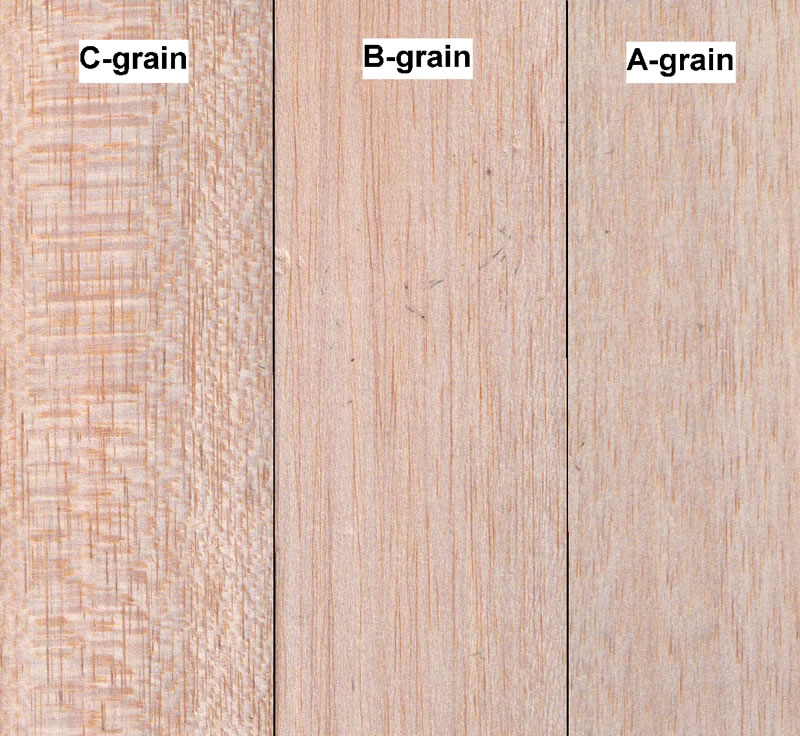
\includegraphics[width=7cm]{balsagrain}
    \caption{Different Grains of Balsa Wood}
    \label{wood}
\end{figure}

\noindent \textbf{B} The following drawing represents the engineering drawing of the most recent iteration of the UAV. \\ 

\newpage

\begin{figure}
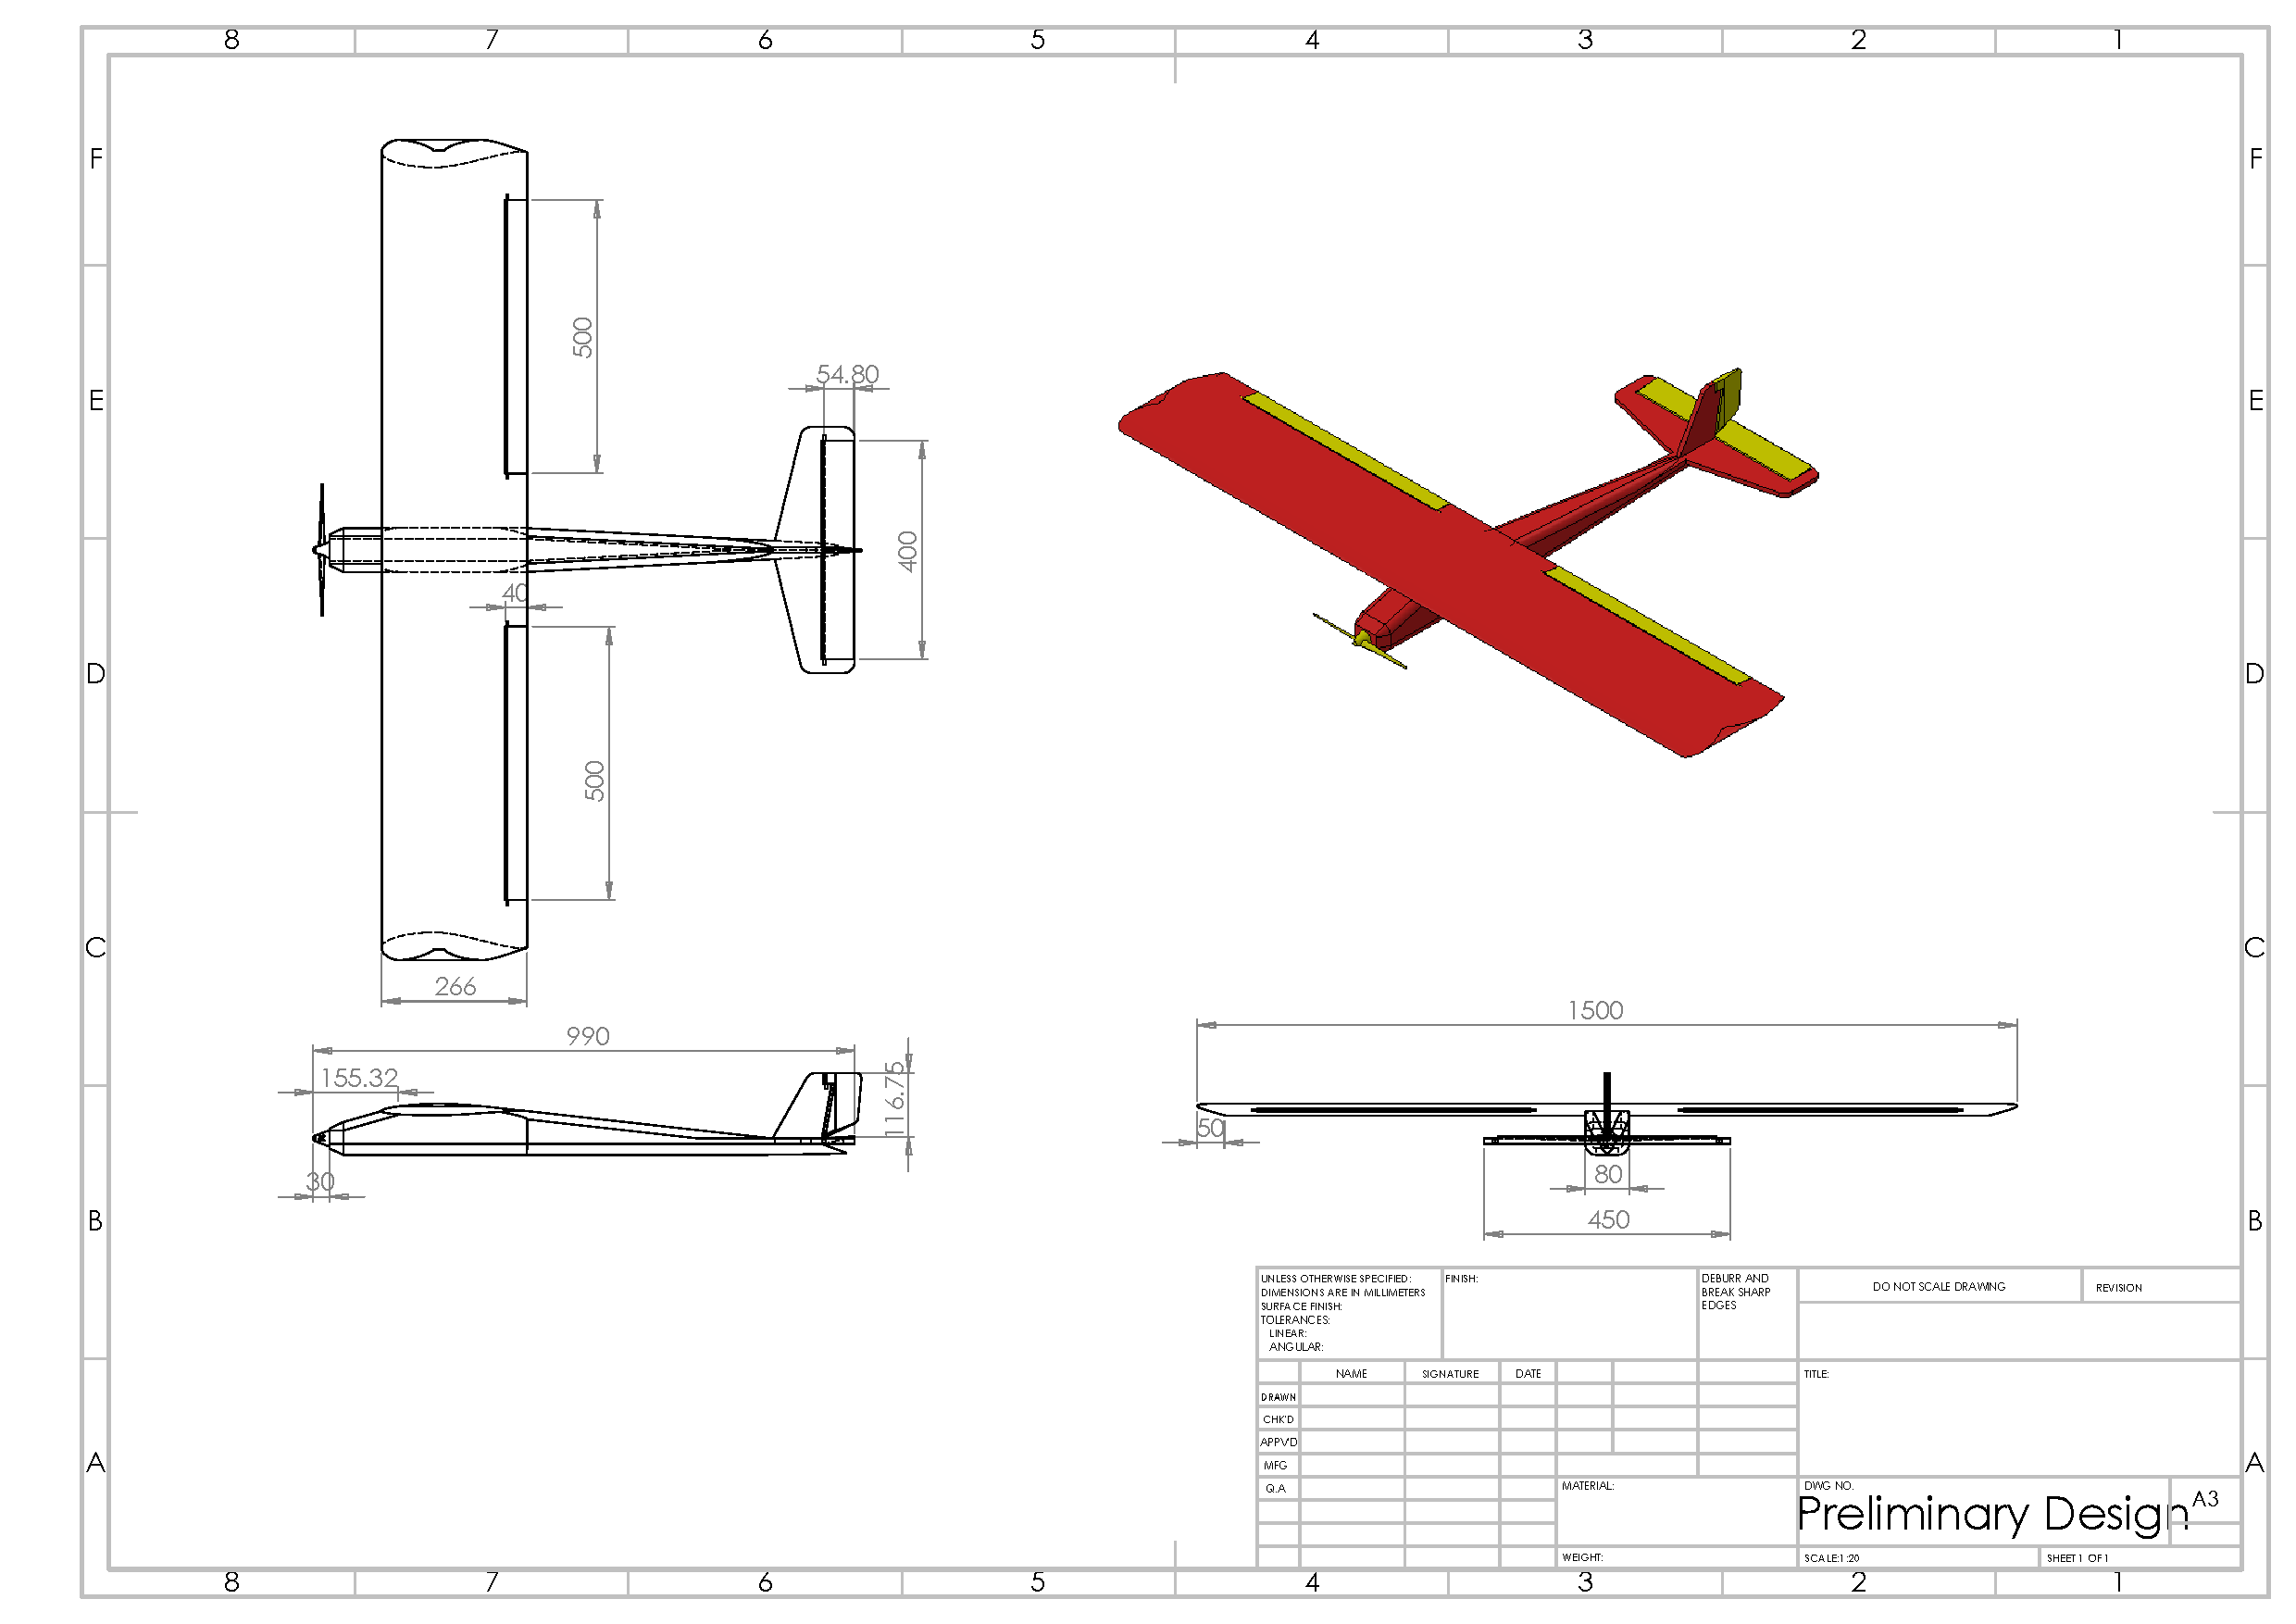
\includepdf{PreliminaryDesignDADA.pdf}
\caption{Engineering Drawing UAV}
\end{figure}

\end{document}